\documentclass[degree=master,tocarialchapter]{thuthesis}
% 选项
%   degree=[bachelor|master|doctor|postdoctor], % 必选,学位类型
%   language=[chinese|english], % 可选(默认:chinese),论文的主要语言
%   secret,                % 可选(默认:关闭),是否有密级
%   tocarialchapter,       % 可选(默认:关闭),章目录中使用黑体(这项表示同时打开下面两项)
%   tocarialchapterentry,  % 可选(默认:关闭),单独控制章标题在目录中使用黑体
%   tocarialchapterpage,   % 可选(默认:关闭),单独控制章页码在目录中使用黑体

% 所有其它可能用到的包都统一放到这里了,可以根据自己的实际添加或者删除。
\usepackage{thuthesis}
\usepackage{tikz}


% 定义所有的图片文件在 figures 子目录下
\graphicspath{{figures/}}

% 可以在这里修改配置文件中的定义。导言区可以使用中文。
% \def\myname{何琦}

\begin{document}

%%% 封面部分
\frontmatter
\thusetup{
  %******************************
  % 注意:
  %   1. 配置里面不要出现空行
  %   2. 不需要的配置信息可以删除
  %******************************
  %
  %=====
  % 秘级
  %=====
  secretlevel={秘密},
  secretyear={10},
  %
  %=========
  % 中文信息
  %=========
  ctitle={基于描述的自动耦合实验实现与验证},
  cdegree={工学学士},
  cdepartment={计算机科学与技术系},
  cmajor={计算机科学与技术},
  cauthor={何琦},
  csupervisor={黄震春副研究员},
  % 日期自动使用当前时间,若需指定按如下方式修改:
  % cdate={超新星纪元},
  %
  %=========
  % 英文信息
  %=========
  etitle={Implementation and verification of Automatic Coupling for Earth System Models based on Description Language},
  % 这块比较复杂,需要分情况讨论:
  % 1. 学术型硕士
  %    edegree:必须为Master of Arts或Master of Science(注意大小写)
  %             “哲学、文学、历史学、法学、教育学、艺术学门类,公共管理学科
  %              填写Master of Arts,其它填写Master of Science”
  %    emajor:“获得一级学科授权的学科填写一级学科名称,其它填写二级学科名称”
  % 2. 专业型硕士
  %    edegree:“填写专业学位英文名称全称”
  %    emajor:“工程硕士填写工程领域,其它专业学位不填写此项”
  % 3. 学术型博士
  %    edegree:Doctor of Philosophy(注意大小写)
  %    emajor:“获得一级学科授权的学科填写一级学科名称,其它填写二级学科名称”
  % 4. 专业型博士
  %    edegree:“填写专业学位英文名称全称”
  %    emajor:不填写此项
  edegree={Scholar of Engineering},
  emajor={Computer Science and Technology},
  eauthor={He Qi},
  esupervisor={Associate Professor Huang Zhenchun},
  % 日期自动生成,若需指定按如下方式修改:
  % edate={December, 2005},
  %
  % 关键词用“英文逗号”分割
}

% 定义中英文摘要和关键字
\begin{cabstract}
  耦合技术是解决气候多模式模拟问题的重要手段。目前已有一种基于顶层驱动的耦合器
  可以对多个模式分量进行全局调度、数据交换、统计分析、自动存储恢复等功能。我们
  通过将已存在的模式分量适配进该耦合器来复现模式分量结果的方式,对该耦合器的功能
  进行验证和改进。
  
  我们选用F2000实验作为我们的复现目标。这个实验主要由4个模式分量和1个数据分量构成,
  其原本的工作模式是由驱动模块启动各个模式分量并进行数据交换,然后各个模块分别进行
  各自独立的计算、存储、统计、恢复等功能。现在,我们将这些分量进行重构,在保持其
  原有的计算机能不改变的情况下,将存储、统计、恢复等功能集成到耦合器来处理。

  重构和复现过程验证了耦合器对各种传统模式分量的适配能力。通过从耦合器进行
  的全局数据分析,我们可以将不同模式分量的数据结合在一起。耦合器全局调度的存储和
  恢复功能确保了整个多模式模拟的同步性和稳定性。对某单一模式分量的插拔实验提供了
  模式分量更新无缝对接和等位模式分量数据比较的功能。

  在重构和适配过程中,我们编写了大量调试工具,其中一部分经过标准化后可以帮助耦合器
  进行调试信息动态输出和错误定位。针对模式分量内部可能出现的错误,我们也提供了一套
  嵌入式调试流程。这些调试工具可以在较短的工作量内定位耦合器配置错误或是确认模式
  分量内部错误。

\end{cabstract}

% 如果习惯关键字跟在摘要文字后面,可以用直接命令来设置,如下:
\ckeywords{地球系统模式, 耦合器, 描述语言, 自动耦合, 可行性验证}

\begin{eabstract}

Coupling technology is an important means to solve the problem of multi-model climate simulation. At present, a coupler based on top-level driver can perform global scheduling, data exchange, statistical analysis, automatic storage recovery and other functions for multiple mode components. We verify and improve the function of the coupler by adapting the existing mode components to the coupler to reproduce the results of the mode components.

We chose F2000 experiment as our recurrence target. This experiment is mainly composed of four mode components and one data component. The original working mode of this experiment is that the driver module starts each mode component and exchanges data. Then each module carries out its own independent calculation, storage, statistics, recovery and other functions. Now, we reconstruct these components and integrate the functions of storage, statistics and recovery into the coupler to deal with them while keeping the original computer unchanged.

The reconstructing and reproducing process verifies the coupler's adaptability to various traditional mode components. By analyzing the global data from the coupler, we can combine the data of different mode components. The storage and recovery function of coupler global scheduling ensures the synchronization and stability of the whole multi-mode simulation. The interpolation experiment of a single mode component provides the function of seamless docking of mode component updating and data comparison of allele mode component.

In the process of reconfiguration and adaptation, we have compiled a large number of debugging tools, some of which are standardized to help couplers to dynamically output debugging information and locate errors. We also provide an embedded debugging process for possible errors within the mode components. These debugging tools can locate coupler configuration errors or confirm mode component internal errors within a relatively short workload.

\end{eabstract}

\ekeywords{Earth System Model, Coupler, Description Language, Automatic Coupling, Feasibility Verification}

% 如果使用授权说明扫描页,将可选参数中指定为扫描得到的 PDF 文件名,例如:
% \makecover[scan-auth.pdf]
\makecover

%% 目录
\tableofcontents

%% 符号对照表
\begin{denotation}[3cm]
\item[CESM] 地球气候系统模式(Community Earth System Model)
\item[NCAR] National Center for Atmospheric Research
\item[CAM] Community Atmosphere Model
\item[CLM] Community Land Model
\item[CICE] Community IceCodE
\item[RTM] River Transport Model
\end{denotation}



% % 也可以使用 nomencl 宏包:

% \printnomenclature[3cm]

% \nomenclature{HPC}{高性能计算 (High Performance Computing)}
% \nomenclature{cluster}{集群}
% \nomenclature{Itanium}{安腾}
% \nomenclature{SMP}{对称多处理}
% \nomenclature{API}{应用程序编程接口}
% \nomenclature{PI}{聚酰亚胺}
% \nomenclature{MPI}{聚酰亚胺模型化合物,N-苯基邻苯酰亚胺}
% \nomenclature{PBI}{聚苯并咪唑}
% \nomenclature{MPBI}{聚苯并咪唑模型化合物,N-苯基苯并咪唑}
% \nomenclature{PY}{聚吡咙}
% \nomenclature{PMDA-BDA}{均苯四酸二酐与联苯四胺合成的聚吡咙薄膜}
% \nomenclature{$\Delta G$}{活化自由能 (Activation Free Energy)}
% \nomenclature{$\chi$}{传输系数 (Transmission Coefficient)}
% \nomenclature{$E$}{能量}
% \nomenclature{$m$}{质量}
% \nomenclature{$c$}{光速}
% \nomenclature{$P$}{概率}
% \nomenclature{$T$}{时间}
% \nomenclature{$v$}{速度}



%%% 正文部分
\mainmatter
\chapter{引言}
\label{cha:intro}

CESM模型是一类应用较为广泛的自然气候变化模型,它包括大气模型,陆地模型,海洋模型等子模型。单个模型专注考虑某一个区域的物理过程,因此在与其他区域的接触面需要提供记录数据或联合其他模型互相提供数据才能尽可能模拟出真实过程。因此一套完整的模型运行流程由多个模型轮流运行互相提供数据组成。

耦合技术是一种专注于多个模型中数据交互的控制技术,其将每个模型封装成模式分量,然后由耦合器控制整体的运行时序、数据交互、存储恢复、统计分析等。其优点在于顶层耦合器封装了模式分量的运行细节,只将所需的数据暴露给分析部分,将底层实现与顶层分析尽可能隔离开来,从而能够平滑地替换不同模式分量,能够以较少的工作量进行不同模型组合的实验,或进行等位模式分量的对照实验。

由于耦合技术的重要性,国家重点研发计划大规模多模式多过程地球系统模式耦合平台研发项目提出了在架构上支持灵活快捷按需耦合的耦合描述方法研究子课题,现在已经设计并编写了一种可配置、基于代码生成的耦合代码生成框架,并已经通过了海气耦合实验验证。

在这一章里,我们将分别介绍CESM的主要框架、代码结构、运行方式,以及已有的基于代码生成的耦合代码生成框架的主要模块、集成功能、接口实现等信息。

\section{CESM}

CESM\texttrademark\footnote{http://www.cesm.ucar.edu/},全称COMMUNITY EARTH SYSTEM MODEL,是由NCAR于1983年创建,作为供更广泛的气候研究界使用的免费全球大气模型。在过去的20年里,NCAR气候与全球动力学(CGD)部门为大学和NCAR科学家提供了一个全面的三维全球大气模型,用于分析和理解全球气候。由于其广泛使用,该模型被指定为社区工具,并被命名为社区气候模型(CCM)。经过20年的研究与发展,CCM的公式已经稳步改进,且运行该模型所需的计算机变得相对便宜且广泛可用,因而该模型在大学界和一些国家实验室中逐渐被广泛使用。

原始CCM模型的局限性在于它不包括全球海洋和海冰模型。因此,在1994年,NCAR科学家提交了一项计划,以国家科学基金会(NSF)开发和使用气候系统模型(CSM),其中包括大气、陆面、海洋和海冰的模型。这些模式分量能够对分量间的通量不进行任何的情况下进行耦合。该计划最初侧重于气候系统的物理方面,然后在随后的版本中追加了生物地球化学插件和高层大气模式分量。该项目的第一阶段是NCAR工作人员开发的模型,之后,模型和相关数据集将提供给科学界。此外,该项目还计划建立一个新的模型和代码社区,让感兴趣的科学界有机会参与CSM的各个方面。这也是我们能够基于该模型进行后续开发和封装的重要条件之一。

\subsection{主要框架}

CESM代码主要分为两部分:模式分量和实例生成脚本包。

模式分量主要分为大气模式分量atm\footnote{atmosphere},海洋模式分量ocn\footnote{ocean},陆地模式lnd\footnote{land},海冰模式ice\footnote{sea-ice},冰川模式glc\footnote{land-ice},海浪模式wav\footnote{ocean-wave},海河径流模式rof\footnote{river-runoff},以及一个专门用于数据交换的模式分量drv\footnote{也作coupler, cpl}。

单个模式分量内部包含多种实现方式。不同实现方式通常含有不同意义,例如采用不同假设、运算核心公式不同、计算精度差异、网格划分和网格密度不同、物理意义不同等等。通常情况下每种模式分量选择且仅选择其中一种实现进行耦合运行。在特定的条件下(如在线比对同一模式分量的多种不同实现方式)可以在单个模式分量中应用多种实现方式同时进行耦合运算,但此种情况下数据处理会变得较通常时更为复杂。另外,如果某些模式分量对于整个实验来说影响很小或是并不关心,可以不采用实现或采用空实现。一般来说,一个以气候模拟为目的的耦合模型通常只采用每种模式的单一实现。

最常见的模式是纯数据模式分量,这种模式分量取 data 首字母 d 开头命名,作用是读取
测量数据用于与其他公式型模式分量进行数据交换,并接收其他模式分量传入的数据与真实数据进行对比做出数据统计
和误差分析。通常来说当单个模式分量要进行适配测试时,会将所有与之直接相连的模式分量设置为纯数据模式分量,
从而确保了待测试分量从其他分量获取的输入值较为准确,可以帮助进行针对待测试分量的耦合运行和数据分析。
而对于与待测分量不直接相连的分量,通常采用空实现以尽可能减少运行时间。另外,在某些综合耦合实验中,若某些
模式分量的实现与其他主要模式分量有较大差异,如实现未完成
\footnote{本文复现的 F2000 实验就是在海洋模式 pop2 未完成的情况下,用 docn 模式代替进行的实验}
,单个模式测试不满足要求,误差量级不符,联合测试不稳定或无法收敛等情况,可以采用纯数据模式分量代替其中不满足条件的分量进行耦合验证
\footnote{需要注意的是,此种情况下耦合模型误差较一个真实模式分量实现偏小,数据分析时应当考虑到这一点}
。

模式分量的主要实现方式取 community 首字母 c 命名,这种模型在CESM社区中广泛使用,经过各种工作人员和科学家的共同开发,以及大量实验验证和改进,通常被认为是该模式分量的 baseline 。实际上,当一个新的模式分量进行耦合测试时,其正确性由于纯数据模式分量的耦合测试来保证,而其实际精度通常根据由社区模型进行耦合而成的模型进行测算。这可以在一定程度上反映该模式分量实现对来自外部误差的敏感程度。另外,该社区模型也会不断采纳来自其他模型的公式进行修正,因而保证了其的即时性和准确度。目前大部分成型的实验都包含相当数量的社区模型作为其模式分量的实现。

另外还有残余模型和死亡模型。前者只有接口而没有具体内容,在耦合模式完全不需要也不读取某个模式分量的数据时使用,最大化运行效率。死亡模型则采用随机的公式进行计算,并将得出的随机结果传输给其他模型。这种模型无法得出有意义的数据和统计结论,通常只用于测试可行性和数据溢出错误处理,或配合其他模型测试运行速度。在实际的耦合实验中,残余模型经常被接入被忽略的部分,而死亡模型不会出现在实际耦合实验中。

驱动模式分量,也作耦合模式分量,是专门用于各个模式分量的数据交换的一个特殊的模式分量。在CESM代码中这个模块是作为一个模式分量来看待的
\footnote{而在我们的代码中,这个模块作为顶层耦合器被独立提出并进行改进以增加适用性}
。
在任何实验中,驱动模式分量必须存在,且每个模式分量都只和驱动模式分量进行通信。因而所有的通信方式都被硬编码为“向驱动模式分量发送数据”和“从驱动模式分量获取数据”。实际上,驱动模式分量也有不同的实现方式
\footnote{常见的包括 cpl\_mct , cpl\_esmf 等}
,而对于每种驱动方式,由于数据传输被硬编码在每个模式分量中,因此每个模式分量的每一个实现都必须对驱动模式分量的每一个实现进行分别硬编码。\footnote{这应该是CESM最严重的缺点之一,也是我们主要要解决的问题}。

\section{字体命令}
\label{sec:first}

苏轼(1037-1101),北宋文学家、书画家。字子瞻,号东坡居士,眉州眉山(今属四川)人
。苏洵子。嘉佑进士。神宗时曾任祠部员外郎,因反对王安石新法而求外职,任杭州通判,
知密州、徐州、湖州。后以作诗“谤讪朝廷”罪贬黄州。哲宗时任翰林学士,曾出知杭州、
颖州等,官至礼部尚书。后又贬谪惠州、儋州。北还后第二年病死常州。南宋时追谥文忠。
与父洵弟辙,合称“三苏”。在政治上属于旧党,但也有改革弊政的要求。其文汪洋恣肆,
明白畅达,为“唐宋八大家”之一。  其诗清新豪健,善用夸张比喻,在艺术表现方面独具
风格。少数诗篇也能反映民间疾苦,指责统治者的奢侈骄纵。词开豪放一派,对后代很有影
响。《念奴娇·赤壁怀古》、《水调歌头·丙辰中秋》传诵甚广。

{\kaishu 坡仙擅长行书、楷书,取法李邕、徐浩、颜真卿、杨凝式,而能自创新意。用笔丰腴
  跌宕,有天真烂漫之趣。与蔡襄、黄庭坚、米芾并称“宋四家”。能画竹,学文同,也喜
  作枯木怪石。论画主张“神似”,认为“论画以形似,见与儿童邻”;高度评价“诗中有
  画,画中有诗”的艺术造诣。诗文有《东坡七集》等。存世书迹有《答谢民师论文帖》、
  《祭黄几道文》、《前赤壁赋》、《黄州寒食诗帖》等。  画迹有《枯木怪石图》、《
  竹石图》等。}

{\fangsong 易与天地准,故能弥纶天地之道。仰以观於天文,俯以察於地理,是故知幽明之故。原
  始反终,故知死生之说。精气为物,游魂为变,是故知鬼神之情状。与天地相似,故不违。
  知周乎万物,而道济天下,故不过。旁行而不流,乐天知命,故不忧。安土敦乎仁,故
  能爱。范围天地之化而不过,曲成万物而不遗,通乎昼夜之道而知,故神无方而易无体。}

% 非本科生一般用不到幼圆与隶书字体。需要的同学请查看 ctex 文档。
{\ifcsname youyuan\endcsname\youyuan\else[无 \cs{youyuan} 字体。]\fi 有天地,然后
  万物生焉。盈天地之间者,唯万物,故受之以屯;屯者盈也,屯者物之始生也。物生必蒙,
  故受之以蒙;蒙者蒙也,物之穉也。物穉不可不养也,故受之以需;需者饮食之道也。饮
  食必有讼,故受之以讼。讼必有众起,故受之以师;师者众也。众必有所比,故受之以比;
  比者比也。比必有所畜也,故受之以小畜。物畜然后有礼,故受之以履。}

{\heiti 履而泰,然后安,故受之以泰;泰者通也。物不可以终通,故受之以否。物不可以终
  否,故受之以同人。与人同者,物必归焉,故受之以大有。有大者不可以盈,故受之以谦。
  有大而能谦,必豫,故受之以豫。豫必有随,故受之以随。以喜随人者,必有事,故受
  之以蛊;蛊者事也。}

{\ifcsname lishu\endcsname\lishu\else[无 \cs{lishu} 字体。]\fi 有事而后可大,故受
  之以临;临者大也。物大然后可观,故受之以观。可观而后有所合,故受之以噬嗑;嗑者
  合也。物不可以苟合而已,故受之以贲;贲者饰也。致饰然后亨,则尽矣,故受之以剥;
  剥者剥也。物不可以终尽,剥穷上反下,故受之以复。复则不妄矣,故受之以无妄。}

{\songti 有无妄然后可畜,故受之以大畜。物畜然后可养,故受之以颐;颐者养也。不养则不
  可动,故受之以大过。物不可以终过,故受之以坎;坎者陷也。陷必有所丽,故受之以
  离;离者丽也。}

\section{表格样本}
\label{chap1:sample:table}

\subsection{基本表格}
\label{sec:basictable}

模板中关于表格的宏包有三个:\pkg{booktabs}、\pkg{array} 和 \pkg{longtabular},命
令有一个 \cs{hlinewd}。三线表可以用 \pkg{booktabs} 提供
的 \cs{toprule}、\cs{midrule} 和 \cs{bottomrule}。它们与 \pkg{longtable} 能很好的
配合使用。如果表格比较简单的话可以直接用命令 \cs{hlinewd}\marg{width} 控制。
\begin{table}[htb]
  \centering
  \begin{minipage}[t]{0.8\linewidth} % 如果想在表格中使用脚注,minipage是个不错的办法
  \caption[模板文件]{模板文件。如果表格的标题很长,那么在表格索引中就会很不美
    观,所以要像 chapter 那样在前面用中括号写一个简短的标题。这个标题会出现在索
    引中。}
  \label{tab:template-files}
    \begin{tabularx}{\linewidth}{lX}
      \toprule[1.5pt]
      {\heiti 文件名} & {\heiti 描述} \\\midrule[1pt]
      thuthesis.ins & \LaTeX{} 安装文件,DocStrip\footnote{表格中的脚注} \\
      thuthesis.dtx & 所有的一切都在这里面\footnote{再来一个}。\\
      thuthesis.cls & 模板类文件。\\
      thuthesis-numeric.bst    & 参考文献 Bib\TeX\ 样式文件。\\
      thuthesis-author-year.bst    & 参考文献 Bib\TeX\ 样式文件。\\
      thuthesis.sty   & 常用的包和命令写在这里,减轻主文件的负担。\\
      \bottomrule[1.5pt]
    \end{tabularx}
  \end{minipage}
\end{table}

首先来看一个最简单的表格。表 \ref{tab:template-files} 列举了本模板主要文件及其功
能。请大家注意三线表中各条线对应的命令。这个例子还展示了如何在表格中正确使用脚注。
由于 \LaTeX{} 本身不支持在表格中使用 \cs{footnote},所以我们不得不将表格放在
小页中,而且最好将表格的宽度设置为小页的宽度,这样脚注看起来才更美观。

\subsection{复杂表格}
\label{sec:complicatedtable}

我们经常会在表格下方标注数据来源,或者对表格里面的条目进行解释。前面的脚注是一种
不错的方法,如果不喜欢脚注,可以在表格后面写注释,比如表~\ref{tab:tabexamp1}。
\begin{table}[htbp]
  \centering
  \caption{复杂表格示例 1。这个引用 \cite{tex} 不会导致编号混乱。}
  \label{tab:tabexamp1}
  \begin{minipage}[t]{0.8\textwidth}
    \begin{tabularx}{\linewidth}{|l|X|X|X|X|}
      \hline
      \multirow{2}*{\diagbox[width=5em]{x}{y}} & \multicolumn{2}{c|}{First Half} & \multicolumn{2}{c|}{Second Half}\\\cline{2-5}
      & 1st Qtr &2nd Qtr&3rd Qtr&4th Qtr \\ \hline
      East$^{*}$ &   20.4&   27.4&   90&     20.4 \\
      West$^{**}$ &   30.6 &   38.6 &   34.6 &  31.6 \\ \hline
    \end{tabularx}\\[2pt]
    \footnotesize 注:数据来源《\thuthesis{} 使用手册》。\\
    *:东部\\
    **:西部
  \end{minipage}
\end{table}

此外,表~\ref{tab:tabexamp1} 同时还演示了另外两个功能:1)通过 \pkg{tabularx} 的
 \texttt{|X|} 扩展实现表格自动放大;2)通过命令 \cs{diagbox} 在表头部分
插入反斜线。

为了使我们的例子更接近实际情况,我会在必要的时候插入一些“无关”文字,以免太多图
表同时出现,导致排版效果不太理想。第一个出场的当然是我的最爱:风流潇洒、骏马绝尘、
健笔凌云的{\heiti 李太白}了。

李白,字太白,陇西成纪人。凉武昭王暠九世孙。或曰山东人,或曰蜀人。白少有逸才,志
气宏放,飘然有超世之心。初隐岷山,益州长史苏颋见而异之,曰:“是子天才英特,可比
相如。”天宝初,至长安,往见贺知章。知章见其文,叹曰:“子谪仙人也。”言于明皇,
召见金銮殿,奏颂一篇。帝赐食,亲为调羹,有诏供奉翰林。白犹与酒徒饮于市,帝坐沉香
亭子,意有所感,欲得白为乐章,召入,而白已醉。左右以水颒面,稍解,援笔成文,婉丽
精切。帝爱其才,数宴见。白常侍帝,醉,使高力士脱靴。力士素贵,耻之,摘其诗以激杨
贵妃。帝欲官白,妃辄沮止。白自知不为亲近所容,恳求还山。帝赐金放还。乃浪迹江湖,
终日沉饮。永王璘都督江陵,辟为僚佐。璘谋乱,兵败,白坐长流夜郎,会赦得还。族人阳
冰为当涂令,白往依之。代宗立,以左拾遗召,而白已卒。文宗时,诏以白歌诗、裴旻剑舞、
张旭草书为三绝云。集三十卷。今编诗二十五卷。\hfill —— 《全唐诗》诗人小传

浮动体的并排放置一般有两种情况:1)二者没有关系,为两个独立的浮动体;2)二者隶属
于同一个浮动体。对表格来说并排表格既可以像图~\ref{tab:parallel1}、
图~\ref{tab:parallel2} 使用小页环境,也可以如图~\ref{tab:subtable} 使用子表格来做。
图的例子参见第~\ref{sec:multifig} 节。

\begin{table}[htbp]
\noindent\begin{minipage}{0.5\textwidth}
\centering
\caption{第一个并排子表格}
\label{tab:parallel1}
\begin{tabular}{p{2cm}p{2cm}}
\toprule[1.5pt]
111 & 222 \\\midrule[1pt]
222 & 333 \\\bottomrule[1.5pt]
\end{tabular}
\end{minipage}%
\begin{minipage}{0.5\textwidth}
\centering
\caption{第二个并排子表格}
\label{tab:parallel2}
\begin{tabular}{p{2cm}p{2cm}}
\toprule[1.5pt]
111 & 222 \\\midrule[1pt]
222 & 333 \\\bottomrule[1.5pt]
\end{tabular}
\end{minipage}
\end{table}

然后就是忧国忧民,诗家楷模杜工部了。杜甫,字子美,其先襄阳人,曾祖依艺为巩令,因
居巩。甫天宝初应进士,不第。后献《三大礼赋》,明皇奇之,召试文章,授京兆府兵曹参
军。安禄山陷京师,肃宗即位灵武,甫自贼中遁赴行在,拜左拾遗。以论救房琯,出为华州
司功参军。关辅饥乱,寓居同州同谷县,身自负薪采梠,餔糒不给。久之,召补京兆府功曹,
道阻不赴。严武镇成都,奏为参谋、检校工部员外郎,赐绯。武与甫世旧,待遇甚厚。乃于
成都浣花里种竹植树,枕江结庐,纵酒啸歌其中。武卒,甫无所依,乃之东蜀就高適。既至
而適卒。是岁,蜀帅相攻杀,蜀大扰。甫携家避乱荆楚,扁舟下峡,未维舟而江陵亦乱。乃
溯沿湘流,游衡山,寓居耒阳。卒年五十九。元和中,归葬偃师首阳山,元稹志其墓。天宝
间,甫与李白齐名,时称李杜。然元稹之言曰:“李白壮浪纵恣,摆去拘束,诚亦差肩子美
矣。至若铺陈终始,排比声韵,大或千言,次犹数百,词气豪迈,而风调清深,属对律切,
而脱弃凡近,则李尚不能历其藩翰,况堂奥乎。”白居易亦云:“杜诗贯穿古今,  尽工尽
善,殆过于李。”元、白之论如此。盖其出处劳佚,喜乐悲愤,好贤恶恶,一见之于诗。而
又以忠君忧国、伤时念乱为本旨。读其诗可以知其世,故当时谓之“诗史”。旧集诗文共六
十卷,今编诗十九卷。

\begin{table}[htbp]
\centering
\caption{并排子表格}
\label{tab:subtable}
\subcaptionbox{第一个子表格}
{
\begin{tabular}{p{2cm}p{2cm}}
\toprule[1.5pt]
111 & 222 \\\midrule[1pt]
222 & 333 \\\bottomrule[1.5pt]
\end{tabular}
}
\hskip2cm
\subcaptionbox{第二个子表格}
{
\begin{tabular}{p{2cm}p{2cm}}
\toprule[1.5pt]
111 & 222 \\\midrule[1pt]
222 & 333 \\\bottomrule[1.5pt]
\end{tabular}
}
\end{table}

不可否认 \LaTeX{} 的表格功能没有想象中的那么强大,不过只要足够认真,足够细致,
同样可以排出来非常复杂非常漂亮的表格。请参看表~\ref{tab:tabexamp2}。
\begin{table}[htbp]
  \centering\dawu[1.3]
  \caption{复杂表格示例 2}
  \label{tab:tabexamp2}
  \begin{tabular}[c]{|m{1.5cm}|c|c|c|c|c|c|}\hline
    \multicolumn{2}{|c|}{Network Topology} & \# of nodes &
    \multicolumn{3}{c|}{\# of clients} & Server \\\hline
    GT-ITM & Waxman Transit-Stub & 600 &
    \multirow{2}{1.5em}{2\%}&
    \multirow{2}{2em}{10\%}&
    \multirow{2}{2em}{50\%}&
    \multirow{2}{1.2in}{Max. Connectivity}\\\cline{1-3}
    \multicolumn{2}{|c|}{Inet-2.1} & 6000 & & & &\\\hline
    \multirow{2}{1.5cm}{Xue} & Rui  & Ni &\multicolumn{4}{c|}{\multirow{2}*{\thuthesis}}\\\cline{2-3}
    & \multicolumn{2}{c|}{ABCDEF} &\multicolumn{4}{c|}{} \\\hline
\end{tabular}
\end{table}

最后就是清新飘逸、文约意赅、空谷绝响的王大侠了。王维,字摩诘,河东人。工书画,与
弟缙俱有俊才。开元九年,进士擢第,调太乐丞。坐累为济州司仓参军,历右拾遗、监察御
史、左补阙、库部郎中,拜吏部郎中。天宝末,为给事中。安禄山陷两都,维为贼所得,服
药阳喑,拘于菩提寺。禄山宴凝碧池,维潜赋诗悲悼,闻于行在。贼平,陷贼官三等定罪,
特原之,责授太子中允,迁中庶子、中书舍人。复拜给事中,转尚书右丞。维以诗名盛于开
元、天宝间,宁薛诸王驸马豪贵之门,无不拂席迎之。得宋之问辋川别墅,山水绝胜,与道
友裴迪,浮舟往来,弹琴赋诗,啸咏终日。笃于奉佛,晚年长斋禅诵。一日,忽索笔作书
数纸,别弟缙及平生亲故,舍笔而卒。赠秘书监。宝应中,代宗问缙:“朕常于诸王坐闻维
乐章,今存几何?”缙集诗六卷,文四卷,表上之。敕答云,卿伯氏位列先朝,名高希代。
抗行周雅,长揖楚辞。诗家者流,时论归美。克成编录,叹息良深。殷璠谓维诗词秀调雅,
意新理惬。在泉成珠,著壁成绘。苏轼亦云:“维诗中有画,画中有诗也。”今编诗四卷。

\begin{longtable}[c]{c*{6}{r}}
\caption{实验数据}\label{tab:performance}\\
\toprule[1.5pt]
 测试程序 & \multicolumn{1}{c}{正常运行} & \multicolumn{1}{c}{同步} & \multicolumn{1}{c}{检查点} & \multicolumn{1}{c}{卷回恢复}
& \multicolumn{1}{c}{进程迁移} & \multicolumn{1}{c}{检查点} \\
& \multicolumn{1}{c}{时间 (s)}& \multicolumn{1}{c}{时间 (s)}&
\multicolumn{1}{c}{时间 (s)}& \multicolumn{1}{c}{时间 (s)}& \multicolumn{1}{c}{
  时间 (s)}&  文件(KB)\\\midrule[1pt]
\endfirsthead
\multicolumn{7}{c}{续表~\thetable\hskip1em 实验数据}\\
\toprule[1.5pt]
 测试程序 & \multicolumn{1}{c}{正常运行} & \multicolumn{1}{c}{同步} & \multicolumn{1}{c}{检查点} & \multicolumn{1}{c}{卷回恢复}
& \multicolumn{1}{c}{进程迁移} & \multicolumn{1}{c}{检查点} \\
& \multicolumn{1}{c}{时间 (s)}& \multicolumn{1}{c}{时间 (s)}&
\multicolumn{1}{c}{时间 (s)}& \multicolumn{1}{c}{时间 (s)}& \multicolumn{1}{c}{
  时间 (s)}&  文件(KB)\\\midrule[1pt]
\endhead
\hline
\multicolumn{7}{r}{续下页}
\endfoot
\endlastfoot
CG.A.2 & 23.05 & 0.002 & 0.116 & 0.035 & 0.589 & 32491 \\
CG.A.4 & 15.06 & 0.003 & 0.067 & 0.021 & 0.351 & 18211 \\
CG.A.8 & 13.38 & 0.004 & 0.072 & 0.023 & 0.210 & 9890 \\
CG.B.2 & 867.45 & 0.002 & 0.864 & 0.232 & 3.256 & 228562 \\
CG.B.4 & 501.61 & 0.003 & 0.438 & 0.136 & 2.075 & 123862 \\
CG.B.8 & 384.65 & 0.004 & 0.457 & 0.108 & 1.235 & 63777 \\
MG.A.2 & 112.27 & 0.002 & 0.846 & 0.237 & 3.930 & 236473 \\
MG.A.4 & 59.84 & 0.003 & 0.442 & 0.128 & 2.070 & 123875 \\
MG.A.8 & 31.38 & 0.003 & 0.476 & 0.114 & 1.041 & 60627 \\
MG.B.2 & 526.28 & 0.002 & 0.821 & 0.238 & 4.176 & 236635 \\
MG.B.4 & 280.11 & 0.003 & 0.432 & 0.130 & 1.706 & 123793 \\
MG.B.8 & 148.29 & 0.003 & 0.442 & 0.116 & 0.893 & 60600 \\
LU.A.2 & 2116.54 & 0.002 & 0.110 & 0.030 & 0.532 & 28754 \\
LU.A.4 & 1102.50 & 0.002 & 0.069 & 0.017 & 0.255 & 14915 \\
LU.A.8 & 574.47 & 0.003 & 0.067 & 0.016 & 0.192 & 8655 \\
LU.B.2 & 9712.87 & 0.002 & 0.357 & 0.104 & 1.734 & 101975 \\
LU.B.4 & 4757.80 & 0.003 & 0.190 & 0.056 & 0.808 & 53522 \\
LU.B.8 & 2444.05 & 0.004 & 0.222 & 0.057 & 0.548 & 30134 \\
EP.A.2 & 123.81 & 0.002 & 0.010 & 0.003 & 0.074 & 1834 \\
EP.A.4 & 61.92 & 0.003 & 0.011 & 0.004 & 0.073 & 1743 \\
EP.A.8 & 31.06 & 0.004 & 0.017 & 0.005 & 0.073 & 1661 \\
EP.B.2 & 495.49 & 0.001 & 0.009 & 0.003 & 0.196 & 2011 \\
EP.B.4 & 247.69 & 0.002 & 0.012 & 0.004 & 0.122 & 1663 \\
EP.B.8 & 126.74 & 0.003 & 0.017 & 0.005 & 0.083 & 1656 \\
\bottomrule[1.5pt]
\end{longtable}

要想用好论文模板还是得提前学习一些 \TeX/\LaTeX{}的相关知识,具备一些基本能力,掌
握一些常见技巧,否则一旦遇到问题还真是比较麻烦。我们见过很多这样的同学,一直以来
都是使用 Word 等字处理工具,以为 \LaTeX{}模板的用法也应该类似,所以就沿袭同样的思
路来对待这种所见非所得的排版工具,结果被折腾的焦头烂额,疲惫不堪。

如果您要排版的表格长度超过一页,那么推荐使用 \pkg{longtable} 或者 \pkg{supertabular}
宏包,模板对 \pkg{longtable} 进行了相应的设置,所以用起来可能简单一些。
表~\ref{tab:performance} 就是 \pkg{longtable} 的示例。

\subsection{其它}
\label{sec:tableother}
如果不想让某个表格或者图片出现在索引里面,请使用命令 \cs{caption*}。
这个命令不会给表格编号,也就是出来的只有标题文字而没有“表~XX”,“图~XX”,否则
索引里面序号不连续就显得不伦不类,这也是 \LaTeX{} 里星号命令默认的规则。

有这种需求的多是本科同学的英文资料翻译部分,如果觉得附录中英文原文中的表格和图
片显示成“表”和“图”不协调的话,一个很好的办法就是用 \cs{caption*},参数
随便自己写,比如不守规矩的表~1.111 和图~1.111 能满足这种特殊需要(可以参看附录部
分)。
\begin{table}[ht]
  \begin{minipage}{0.4\linewidth}
    \centering
    \caption*{表~1.111\quad 这是一个手动编号,不出现在索引中的表格。}
    \label{tab:badtabular}
      \framebox(150,50)[c]{\thuthesis}
  \end{minipage}%
  \hfill%
  \begin{minipage}{0.4\linewidth}
    \centering
    \caption*{Figure~1.111\quad 这是一个手动编号,不出现在索引中的图。}
    \label{tab:badfigure}
    \framebox(150,50)[c]{薛瑞尼}
  \end{minipage}
\end{table}

如果的确想让它编号,但又不想让它出现在索引中的话,目前模板上不支持。

最后,虽然大家不一定会独立使用小页,但是关于小页中的脚注还是有必要提一下。请看下
面的例子。

\begin{minipage}[t]{\linewidth-2\parindent}
  柳宗元,字子厚(773-819),河东(今永济县)人\footnote{山西永济水饺。},是唐代
  杰出的文学家,哲学家,同时也是一位政治改革家。与韩愈共同倡导唐代古文运动,并称
  韩柳\footnote{唐宋八大家之首二位。}。
\end{minipage}

唐朝安史之乱后,宦官专权,藩镇割据,土地兼并日渐严重,社会生产破坏严重,民不聊生。柳宗
元对这种社会现实极为不满,他积极参加了王叔文领导的“永济革新”,并成为这一
运动的中坚人物。他们革除弊政,打击权奸,触犯了宦官和官僚贵族利益,在他们的联合反
扑下,改革失败了,柳宗元被贬为永州司马。

\section{定理环境}
\label{sec:theorem}

给大家演示一下各种和证明有关的环境:

\begin{assumption}
待月西厢下,迎风户半开;隔墙花影动,疑是玉人来。
\begin{align}
  \label{eq:eqnxmp}
  c & = a^2 - b^2 \\
    & = (a+b)(a-b)
\end{align}
\end{assumption}

千辛万苦,历尽艰难,得有今日。然相从数千里,未曾哀戚。今将渡江,方图百年欢笑,如
何反起悲伤?(引自《杜十娘怒沉百宝箱》)

\begin{definition}
子曰:「道千乘之国,敬事而信,节用而爱人,使民以时。」
\end{definition}

千古第一定义!问世间、情为何物,只教生死相许?天南地北双飞客,老翅几回寒暑。欢乐趣,离别苦,就中更有痴儿女。
君应有语,渺万里层云,千山暮雪,只影向谁去?

横汾路,寂寞当年箫鼓,荒烟依旧平楚。招魂楚些何嗟及,山鬼暗谛风雨。天也妒,未信与,莺儿燕子俱黄土。
千秋万古,为留待骚人,狂歌痛饮,来访雁丘处。

\begin{proposition}
 曾子曰:「吾日三省吾身 —— 为人谋而不忠乎?与朋友交而不信乎?传不习乎?」
\end{proposition}

多么凄美的命题啊!其日牛马嘶,新妇入青庐,奄奄黄昏后,寂寂人定初,我命绝今日,
魂去尸长留,揽裙脱丝履,举身赴清池,府吏闻此事,心知长别离,徘徊庭树下,自挂东南
枝。

\begin{remark}
天不言自高,水不言自流。
\begin{gather*}
\begin{split}
\varphi(x,z)
&=z-\gamma_{10}x-\gamma_{mn}x^mz^n\\
&=z-Mr^{-1}x-Mr^{-(m+n)}x^mz^n
\end{split}\\[6pt]
\begin{align} \zeta^0&=(\xi^0)^2,\\
\zeta^1 &=\xi^0\xi^1,\\
\zeta^2 &=(\xi^1)^2,
\end{align}
\end{gather*}
\end{remark}

天尊地卑,乾坤定矣。卑高以陈,贵贱位矣。 动静有常,刚柔断矣。方以类聚,物以群分,
吉凶生矣。在天成象,在地成形,变化见矣。鼓之以雷霆,润之以风雨,日月运行,一寒一
暑,乾道成男,坤道成女。乾知大始,坤作成物。乾以易知,坤以简能。易则易知,简则易
从。易知则有亲,易从则有功。有亲则可久,有功则可大。可久则贤人之德,可大则贤人之
业。易简,而天下矣之理矣;天下之理得,而成位乎其中矣。

\begin{axiom}
两点间直线段距离最短。
\begin{align}
x&\equiv y+1\pmod{m^2}\\
x&\equiv y+1\mod{m^2}\\
x&\equiv y+1\pod{m^2}
\end{align}
\end{axiom}

《彖曰》:大哉乾元,万物资始,乃统天。云行雨施,品物流形。大明始终,六位时成,时
乘六龙以御天。乾道变化,各正性命,保合大和,乃利贞。首出庶物,万国咸宁。

《象曰》:天行健,君子以自强不息。潜龙勿用,阳在下也。见龙再田,德施普也。终日乾
乾,反复道也。或跃在渊,进无咎也。飞龙在天,大人造也。亢龙有悔,盈不可久也。用九,
天德不可为首也。   

\newcommand\dif{\mathop{}\!\mathrm{d}}
\begin{lemma}
《猫和老鼠》是我最爱看的动画片。
\begin{multline*}%\tag*{[a]} % 这个不出现在索引中
\int_a^b\biggl\{\int_a^b[f(x)^2g(y)^2+f(y)^2g(x)^2]
 -2f(x)g(x)f(y)g(y)\dif x\biggr\}\dif y \\
 =\int_a^b\biggl\{g(y)^2\int_a^bf^2+f(y)^2
  \int_a^b g^2-2f(y)g(y)\int_a^b fg\biggr\}\dif y
\end{multline*}
\end{lemma}

行行重行行,与君生别离。相去万余里,各在天一涯。道路阻且长,会面安可知。胡马依北
风,越鸟巢南枝。相去日已远,衣带日已缓。浮云蔽白日,游子不顾返。思君令人老,岁月
忽已晚。  弃捐勿复道,努力加餐饭。

\begin{theorem}\label{the:theorem1}
犯我强汉者,虽远必诛\hfill —— 陈汤(汉)
\end{theorem}
\begin{subequations}
\begin{align}
y & = 1 \\
y & = 0
\end{align}
\end{subequations}
道可道,非常道。名可名,非常名。无名天地之始;有名万物之母。故常无,欲以观其妙;
常有,欲以观其徼。此两者,同出而异名,同谓之玄。玄之又玄,众妙之门。上善若水。水
善利万物而不争,处众人之所恶,故几于道。曲则全,枉则直,洼则盈,敝则新,少则多,
多则惑。人法地,地法天,天法道,道法自然。知人者智,自知者明。胜人者有力,自胜
者强。知足者富。强行者有志。不失其所者久。死而不亡者寿。

\begin{proof}
燕赵古称多感慨悲歌之士。董生举进士,连不得志于有司,怀抱利器,郁郁适兹土,吾
知其必有合也。董生勉乎哉?

夫以子之不遇时,苟慕义强仁者,皆爱惜焉,矧燕、赵之士出乎其性者哉!然吾尝闻
风俗与化移易,吾恶知其今不异于古所云邪?聊以吾子之行卜之也。董生勉乎哉?

吾因子有所感矣。为我吊望诸君之墓,而观于其市,复有昔时屠狗者乎?为我谢
曰:“明天子在上,可以出而仕矣!” \hfill —— 韩愈《送董邵南序》
\end{proof}

\begin{corollary}
  四川话配音的《猫和老鼠》是世界上最好看最好听最有趣的动画片。
\begin{alignat}{3}
V_i & =v_i - q_i v_j, & \qquad X_i & = x_i - q_i x_j,
 & \qquad U_i & = u_i,
 \qquad \text{for $i\ne j$;}\label{eq:B}\\
V_j & = v_j, & \qquad X_j & = x_j,
  & \qquad U_j & u_j + \sum_{i\ne j} q_i u_i.
\end{alignat}
\end{corollary}

迢迢牵牛星,皎皎河汉女。
纤纤擢素手,札札弄机杼。
终日不成章,泣涕零如雨。
河汉清且浅,相去复几许。
盈盈一水间,脉脉不得语。

\begin{example}
  大家来看这个例子。
\begin{equation}
  \label{ktc}
  \begin{cases}
    \nabla f(\bm{x}^*) - \sum_{j=1}^p \lambda_j \nabla g_j(\bm{x}^*)
      = 0 \\[0.3cm]
    \lambda_j g_j(\bm{x}^*) = 0, \quad j = 1, 2, \dots, p \\[0.2cm]
    \lambda_j \ge 0, \quad j = 1, 2, \dots, p.
  \end{cases}
\end{equation}
\end{example}

\begin{exercise}
  请列出 Andrew S. Tanenbaum 和 W. Richard Stevens 的所有著作。
\end{exercise}

\begin{conjecture} \textit{Poincare Conjecture} If in a closed three-dimensional
  space, any closed curves can shrink to a point continuously, this space can be
  deformed to a sphere.
\end{conjecture}

\begin{problem}
 回答还是不回答,是个问题。
\end{problem}

如何引用定理~\ref{the:theorem1} 呢?加上 \cs{label} 使用 \cs{ref} 即可。妾发
初覆额,折花门前剧。郎骑竹马来,绕床弄青梅。同居长干里,两小无嫌猜。 十四为君妇,
羞颜未尝开。低头向暗壁,千唤不一回。十五始展眉,愿同尘与灰。常存抱柱信,岂上望夫
台。 十六君远行,瞿塘滟滪堆。五月不可触,猿声天上哀。门前迟行迹,一一生绿苔。苔深
不能扫,落叶秋风早。八月蝴蝶来,双飞西园草。感此伤妾心,坐愁红颜老。

\section{参考文献}
\label{sec:bib}
当然参考文献可以直接写 \cs{bibitem},虽然费点功夫,但是好控制,各种格式可以自己随意改
写。

本模板推荐使用 BIB\TeX,分别提供数字引用(\texttt{thuthesis-numeric.bst})和作
者年份引用(\texttt{thuthesis-author-year.bst})样式,基本符合学校的参考文献格式
(如专利等引用未加详细测试)。看看这个例子,关于书的~\cite{tex, companion,
  ColdSources},还有这些~\cite{Krasnogor2004e, clzs, zjsw},关于杂志
的~\cite{ELIDRISSI94, MELLINGER96, SHELL02},硕士论文~\cite{zhubajie,
  metamori2004},博士论文~\cite{shaheshang, FistSystem01},标准文
件~\cite{IEEE-1363},会议论文~\cite{DPMG,kocher99},技术报告~\cite{NPB2},电子文
献~\cite{chuban2001,oclc2000}。
若使用著者-出版年制,中文参考文献~\cite{cnarticle}应增加
\texttt{key=\{pinyin\}} 字段,以便正确进行排序~\cite{cnproceed}。
另外,如果对参考文献有不如意的地方,请手动修改 \texttt{bbl} 文件。

有时候不想要上标,那么可以这样~\inlinecite{shaheshang},这个非常重要。

有时候一些参考文献没有纸质出处,需要标注 URL。缺省情况下,URL 不会在连字符处断行,
这可能使得用连字符代替空格的网址分行很难看。如果需要,可以将模板类文件中
\begin{verbatim}
\RequirePackage{hyperref}
\end{verbatim}
一行改为:
\begin{verbatim}
\PassOptionsToPackage{hyphens}{url}
\RequirePackage{hyperref}
\end{verbatim}
使得连字符处可以断行。更多设置可以参考 \texttt{url} 宏包文档。

\section{公式}
\label{sec:equation}
\renewcommand\vec{\symbf}
\newcommand\mat{\symbf}
贝叶斯公式如式~(\ref{equ:chap1:bayes}),其中 $p(y|\vec{x})$ 为后验;
$p(\vec{x})$ 为先验;分母 $p(\vec{x})$ 为归一化因子。
\begin{equation}
\label{equ:chap1:bayes}
p(y|\vec{x}) = \frac{p(\vec{x},y)}{p(\vec{x})}=
\frac{p(\vec{x}|y)p(y)}{p(\vec{x})}
\end{equation}

论文里面公式越多,\TeX{} 就越 happy。再看一个 \pkg{amsmath} 的例子:
\newcommand{\envert}[1]{\left\lvert#1\right\rvert}
\begin{equation}\label{detK2}
\det\mat{K}(t=1,t_1,\dots,t_n)=\sum_{I\in\vec{n}}(-1)^{\envert{I}}
\prod_{i\in I}t_i\prod_{j\in I}(D_j+\lambda_jt_j)\det\vec{A}
^{(\lambda)}(\overline{I}|\overline{I})=0.
\end{equation}

前面定理示例部分列举了很多公式环境,可以说把常见的情况都覆盖了,大家在写公式的时
候一定要好好看 \pkg{amsmath} 的文档,并参考模板中的用法:
\begin{multline*}%\tag{[b]} % 这个出现在索引中的
\int_a^b\biggl\{\int_a^b[f(x)^2g(y)^2+f(y)^2g(x)^2]
 -2f(x)g(x)f(y)g(y)\dif x\biggr\}\dif y \\
 =\int_a^b\biggl\{g(y)^2\int_a^bf^2+f(y)^2
  \int_a^b g^2-2f(y)g(y)\int_a^b fg\biggr\}\dif y
\end{multline*}

其实还可以看看这个多级规划:
\begin{equation}
  \label{bilevel}
  \begin{cases}
    \max_{\bm{x}} F(\bm{x}, y_1^*, y_2^*, \dots, y_m^*) \\
      \text{subject to:} \\
      \qquad G(\bm{x}) \le 0 \\
      \qquad (y_1^*, y_2^*, \dots, y_m^*) \text{ solves problems }
        (i = 1, 2, \dots, m) \\
      \qquad
        \begin{cases}
          \max_{\bm{x}} f_i(\bm{x}, y_1, y_2, \dots, y_m) \\
          \text{subject to:} \\
          \qquad g_i(\bm{x}, y_1, y_2, \dots, y_m) \le 0.
        \end{cases}
  \end{cases}
\end{equation}
这些跟规划相关的公式都来自于刘宝碇老师《不确定规划》的课件。

\chapter{耦合模式分量适配}
\label{cha:refactor}

\section{结构介绍}

CESM 的各个模式分量由不同研究方向的科学家、工作人员以及部分社区开发人员编写,其代码结构和风格具有较大差异。出于适配和后续调试考虑,我们希望将这些代码尽可能在适配后拥有共通的编译结构、相似的代码结构和对调试工具的较好适应性。为此,我们需要对各个模式分量的代码实现进行分析和调整。

\subsection{cam}

cam 是模式分量 atm 的一种实现。该模式分量实现是在各个耦合实验中最为广泛使用的模式分量实现,也是对耦合框架的主要需求方。在 cam 的代码内部内嵌了足以自行抽取其他模式分量实现独立编译为一个完整耦合实验的代码,这使得 cam 内部实质上包含了顶层耦合框架提供的所有功能的下位或等位替代,可以作为耦合框架编写和调整的参考。然而,在我们的隔离设计中并不希望单个耦合模式分量需要考虑独立获取其他所需的模式分量实现所需信息,直至编译整个耦合实验。因此,我们最终封装后的模式分量实现需要把这部分内嵌依赖和编译代码移除,在必要的部分插入顶层耦合框架作为插件,其他部分则以脚本等形式进行存档或直接单独封装为独立的外部库。

bld 目录存放了上述需求获取和全面编译的代码。这些脚本大部分采用 csh (C-shell, https://en.wikipedia.org/wiki/C\_Shell) 和 perl (http://www.perl.org/) 语言进行执行,其依赖库直接放在了该目录下的 perl5lib 子目录中,配置文件则位于 config\_files 子目录下并以 xml 文件的形式存放。这些配置文件和脚本涉及了各个预置编译平台、各个预置耦合实验的分辨率、各个模块版本和内置物理参数等信息,还包括依赖的各个直接或间接连接的模式分量实现所需的配置信息。在编译完成后, build-namelist 脚本负责基于编译依赖信息和预置配置文件生成一套运行时配置文件,这种结构可以减少在不同模式下切换时带来的不必要的重复编译环节。在我们重构和适配后的版本中,这些运行时配置文件将会由顶层耦合框架生成,但考虑到各个模式分量实现读取的运行时配置格式不尽相同,这里需要将 build-namelist 代码重构为一个读取来自于顶层耦合框架的配置文件并将其格式转变为对应耦合模式分量实现代码运行时可读格式的配置文件。实际上,在该工作完成后,我们鼓励新的耦合模式分量实现都按照预设的顶层耦合框架配置文件进行读取的设计,这样可以直接跳过生成 namelist 运行时配置的步骤以达到简化适配流程的结果。为此,顶层耦合框架配置文件应当具有足够的适应性并能够提取各个模式分量中的共同配置进行同步以防止数据不匹配等问题。另外,考虑到整个模式分量实现的代码均由 fortran 代码构成, python 部分仅参与代码生成部分而不接触实际运行,这里的配置文件采用 fortran 语言内置的 namelist 格式。该格式是一种人类可读的类字典复合格式,具有相当的适配性和可读性,易于调试。其缺点在于运行时配置的读取较二进制文件较慢且难以并行,但考虑到目前耦合模式分量的运行时配置相对较少,实际进行速度测试时该部分效率影响可以忽略不计,故暂时维持 CESM 设定的格式。未来若存在接入 C 或 C++ 等其他语言代码需求则可以考虑采用更加效率重视型的 NetCDF 文件甚至直接通过 protobuf (Google Protocol Buffer, https://developers.google.com/protocol-buffers/)进行在线的数据传输。该目录还存放编译过程中产生的中间结果以支持基于 Makefile 的增量编译等特性。

chem\_proc 目录存放与化学过程插件相关的源代码及独立测试框架。化学过程插件是在社区中被提出的一个专门处理大气模式中涉及到的纯化学和化学相关过程的插件,自身具有独立的公式体系并可以单独进行编译和运行。其调试过程将预置的接口参数作为输入从文件中读取,运行化学过程后将输出写入文件中并通过脚本进行外部读取从而和观测数据进行对比从而确认代码正确性。实际与 cam 共同编译时,输入输出部分被移除,成为一个独立的内部库与 cam 源码一起编译。这种分阶段调试的方式可以极大地降低错误定位难度,我们在其他的模式分量实现中也会看到类似的处理方法。但相对的,这种方法需要对实际物理数据进行分析处理以获取该化学过程需要的输入输出数据,因此需要相应的气候地理学家的支持。对于从纯代码角度进行封装和适配的角度来说,由于代码隔离的过程中需要生成中间数据,因此数据的正确性对另一部分代码存在依赖,因而不能完全隔离两部分代码的正确性。从结果上看,在封装的过程中我们只保留了原有的代码隔离模块,并没有再对耦合模式分量实现中的已有代码进行拆分解耦。

src 目录存放了 cam 主要部分的全部源码。这部分源码的内部依赖较为复杂且难以拆分,因此我们选择将其作为黑盒进行处理。这里 cam 的对外接口主要是 cpl\_esmf 、 cpl\_mct 、 cpl\_share 三个目录,其中由于我们采用了 MCT 作为基本数据结构,因此主要接口为 cpl\_mct 目录下的 atm\_comp\_mct.F90 文件。 cpl\_share 目录提供了 MCT 数据结构的域定义和编号缓存,以减小多进程高频率的数据结构访问下带来的字符串操作对应延迟,最大化运行效率。这两个目录是我们封装过程中主要需要处理的部分。另外,代码各个涉及到错误处理的部分都要求与顶层耦合调试工具进行对接,因此还涉及数个需要调整的代码段。在针对 cam 模块进行的错误定位时,通常可以通过在内部控制模块 control 设置断点来进行大致定位并进一步调试。

test 目录提供了一套以 cam 为中心进行单元测试的模块,其测试范围包括 cam 独立运行和各种包含 cam 的耦合试验测试。由于我们对接口进行了适配修改,因此将 cam 作为整体的测试(包括对 cam 的封装级测试和对于带 cam 的外部耦合试验实例整体测试)由于接口发生变化而需要修改或直接放弃而无法运行,但针对 cam 各个内部模块的小规模测试依然成立,可以防止进行嵌入式修改后造成的数值不匹配或计算逻辑错误。

tools 目录提供了一些辅助调试的工具,主要用于不同格式的输入文件和数据文件之间的互相转换。顶层耦合中的部分代码和工具参考了这部分代码并进行了对各个模式分量的适配使得他们可以用于全部的模式分量实现中的格式转换。

总体上来看, cam 的代码结构是所有模式分量实现中较为复杂的一个。出于适配效率考虑我们并没有完整地分析其中的具体结构细节或是实现细节,而是尽可能将其作为一个可编译运行的整体来进行封装和适配来尽可能在保证其正确性和完整性的情况下减少适配工作量。值得一提的是,由于 cam 部分结构并不具有普适性且复杂度偏高,我们并没有采用该结构作为适配后的结构,而是参考了之后更为简洁和标准化的模式分量结构。在 cam 的适配过程中向目标结构进行了一定的修改的同时保留了 cam 部分框架特点以尽可能为 cam 模式分量实现的更新版适配做准备。

\subsection{pop2}

pop2 是海洋模式分量 ocn 的一个实现。该模式分量实现并不包含于我们要复现的 F2000 实验中,但其结构为我们进行其他模式分量封装提供了很大帮助,因此这里着重介绍一下 pop2 模式分量实现的结构。

与 cam 类似,pop2 提供了 bld 目录作为基于 csh 和 perl 脚本语言的共通编译框架,其内部结构与 cam 类似但更精简,且与我们的适配关系不大,在此不再赘述。但 pop2 模式分量实现在编写时还提供了另一套独立的自编译框架,该框架位于 build 目录下,并可以在没有外部依赖的情况下独立完成对 pop2 源代码的编译。这种编译框架能够极大的方便适配过程中进行的隔离编译和隔离调试,因此我们以该目录为模板对所有涉及的模式分量进行了附加自编译模块。特别的,对于 cam 模式分量来说,其编译系统较为复杂,直接插入附加自编译模块导致了部分冲突和重复编译,因此我们只对 cam 模式分量进行了特殊适配,保留了其原有的编译系统的基础上,将删减过的自编译模块以脚本调用的形式附加,从而保证了编译效率和正确性。

build 目录下提供了大量配置文件以在各个预设实验平台下编译。由于我们的实验平台并非预设平台,因此要对这些配置文件进行修改。我们选择了与实验平台较为接近的 linux 配置并对其进行了针对实验平台的改动,包括修改 NetCDF 等依赖库的配置路径,将顶层耦合模块提供的预设配置插入编译选项,设置 mpi 等依赖库的配置开关等。特别需要注意的是,耦合模式分量实现本身没有 C/C++ 代码,但这里必须要对 C++ 编译器进行配置,原因是 fortran 编译器处理部分宏存在问题,需要用 C++ 编译器进行不编译只展开宏的处理,并将处理后的代码放置在 compile 目录下再用 fortran 编译器进行整体编译。另外,默认配置下 fortran 编译器不具有多进程功能,而整个耦合实验必须在 mpi 的多进程模式下进行运行。因此这里编译器需要改为 mpif90 并可以将与单线程 mpi 相关的 mpi-serial 部分全部移除以提高编译效率。另外,当进行嵌入式调试时,调试信息可以被插入 compile 目录下宏展开后的代码以达成自动更新。该自编译模块的主要编译流程如下:

\begin{itemize}
  \item [1)] 
通过外部宏 ARCH 设定编译平台,载入对应的配置文件
  \item [2)]
通过外部宏 SRCDIR 和 EXEDIR 设定源码路径(通常为上级目录)和编译目标路径(通常为 build 目录本身)
  \item [3)]
调用 preprocess.mk 模块进行预编译,将所有找到的源码进行宏展开并放置到 compile 目录下
  \item [4)]
调用 depends.mk 和 fdepends.awk 生成编译所需的依赖
  \item [5)]
调用 compile.mk 依据所生成的依赖自动编译 compile 目录下的所有源码
  \item [6)]
将编译好的源码进行后续处理、打包并与顶层耦合平台对接
\end{itemize}

在上述步骤中,前两步的宏设置可以通过相对路径进行自动适配,因而可以自然应用到各个模式分量实现中。第三步预编译步骤会在若干指定目录下将所有找到的 fortran 代码全部进行宏展开,因此需要针对各个模式分量实现的路径框架进行修改。特别的,对于部分提供多种适配代码的模式分量实现(例如 pop2 同时提供了单进程和多进程的外部库,且他们的接口名称和格式都完全相同),只能选择正确的版本进行预编译,否则会产生重名、冲突、适配错误等情况。预编译中,所有预设的宏都会被展开,因此可以在 compile 文件查看宏展开后的代码来确定是否所有的配置都被正确应用。第四部依赖自动生成设定上只考虑内部依赖,因此对于涉及的外部库 (包括顶层耦合提供的库函数和外部依赖库函数) 都需要在 fdepends.awk 文件进行注册(该文件是 linux 原生的字符串操作脚本语言 awk ,推荐使用 \href{https://www.gnu.org/software/gawk/manual/gawk.html#Getting-Started}{gawk} 进行运行)。生成的依赖文件将被放在 compile 目录的 depends 子目录下,并与第三部生成的宏展开后的代码一同进入第五步编译。这一步作为主要编译步骤,其所需的全部信息都在配置文件和之前的步骤准备完毕,因此可以进行全自动编译。在编译完成后,我们将编译生成的 .o 文件进行打包成为静态库,并将接口相关的 .mod 头文件自动传输至顶层耦合平台以备其他模块(主要是耦合代码核心模块 cpl )编译时使用。总体来说,只需要对平台进行一次配置和一次外部依赖配置,对各个模式分量实现进行代码框架目录设置,即可完成自动编译,因此该模块被我们作为耦合模式分量适配的主要模块来使用。

pop2 的主要代码实现部分由于并没有在 F2000 中使用,故略过不提。这里补充说明一些在 pop2 目录中可以被用来帮助其他模式分量实现进行封装或辅助调试的部分。 mpi 和 serial 目录分别对应多线程和单线程的 mpi 封装接口,在部分需要越过 MCT 层直接调用 mpi 进行操作的场合可以运用这些接口进行调用 (通常是用来调试)。 input\_templates 目录提供了各个分辨率的模板可以用于测试各种边界情况。 test 目录和 tools 目录提供了部分关于时间管理、历史记录和存储恢复的代码。实际上,各个模式分量实现的时间管理模块具有一定的相似性,因此我们提取了其中的共同部分,并加入了一些封装和额外功能作为顶层耦合模式的主时钟。这些代码都为顶层耦合实现的设计提供了参考。

\subsection{docn}

docn 是 ocn 模式分量的纯数据实现,也是 F2000 中唯一一个纯数据模式分量实现。顶层耦合模块的第一版耦合测试就是通过 cam 模块和该模块两个模式分量实现进行耦合完成的。其代码结构在所有的模式分量实现中最为简单,在封装中我们直接将其压缩为单个文件以最大程度上降低该模块可能产生的错误,从而把耦合模式分量调试集中到顶层耦合模块与 cam 模块之间的接口和数据交互中。

虽然核心代码只有一个文件,但作为一个完整的模式分量实现, docn 依然包含一套完整的模式分量实现结构:编译目录 bld , 对两种耦合模式分量实现的接口 cpl\_mct 和 cpl\_esmf ,以及进行独立调试和输入输出的测试工具 tools 目录。值得一提的是, docn 的运行时配置文件 namelist 被拆分为 docn\_in 和 docn\_ocn\_in 两个文件,将专属于该模式分量实现的配置独立出来,以和其他 ocn 模式分量实现的运行时配置保持格式一致。另外,这里接口代码 cpl\_mct 的部分数据适配被移动到了核心代码 docn\_comp\_mod.F90 下,因此在适配过程中会与其他模式分量产生些许不同,我们会在下一章适配过程中详细描述这一部分。

总的来说,选择 docn 作为耦合实验实例的一部分不仅提供了更加简单和模块化的调试顶层耦合模块的流程,还为之后其他实验的纯数据模式分量适配提供了参照。

\subsection{clm}

clm 是 lnd 模式分量的一个实现。该模式分量的特点在于有 clm4\_0 和 clm4\_5 两个等位模块,这两部分分别适用于不同的耦合实验实例,因此需要在配置时进行分别配置。每个等位模块内部将物理、化学和主过程进行了分离。这里的 bld 目录在适配入 pop2 的 build 自编译模块后其编译功能可以被舍弃,从而只需保留生成运行时配置文件的代码。

在实际适配中, lnd 模式分量遇到的主要问题是网格化后的边界处不满一格进行的处理需要顶层耦合模块的 fraction 框架与模式分量进行适配(实际上 ocn 模式分量也有类似问题,但 docn 模式分量没有输入需求因此不需考虑这一点)。为此,在 cpl\_mct 中的 lnd\_domain\_mct 函数中需要直接对 fraction 代码进行修改,使其能够从顶层耦合模型的配置中读取原本从文件中输入的网格大小和网格比例数据。

\subsection{cice}

cice 是 ice 模式分量的一个实现。该模式分量比上述模式分量的实现较为简单且有较为详细的文档。与 clm 类似的,这里只保留 bld 目录下进行运行时配置文件 namelist 生成的部分代码,编译部分同样交给自编译模块 build 。代码目录 src 提供了 mpi 的单进程和多进程接口, driver 目录下的 cice4 提供了一套能够独立运行和调试 cice 自身的驱动接口,其中 init , run , final 分别对应于 driver 接口中的三个接口,而 history 和 restart 分别对应顶层耦合模式的主时钟模块的两个功能历史记录和存储恢复。这部分代码作为独立调试使用,在最终模式分量编译和封装时不加入编译的源码目录列表。

在 cice 模块的 cpl\_share 目录下存放了与 cice4 同名同接口不同实现的模块。这些模块移除了调试并加入了 NetCDF , ParallelIO 等多进程/线程加速代码以提高运行效率。在实际开发中,可以在 cice4 接口进行调试通过后,将其同步到 cpl\_share 接口中以确保多线程代码的正确性,并将加速代码代替 cice4 进行完整的库编译以达成隔离调试和运行提速。如果最终编译出现问题,则需要检查替换的多进程部分是否会出现数据不匹配或 race condition 等问题。

总体来说, cice 作为一个结构较为简单的模式分量实现,其自带详细的文档和独立调试模块,使得其独立适配难度较低。事实上,cice 和 docn 两模块构成的简单耦合实验实例相较 cam 和 docn 的耦合实验实例从代码层面上更加适合对顶层耦合模式进行调试,但 ice 和 ocn 模式分量对 atm 模式的输出存在较多依赖,因此需要追加 datm 模块才能较好地保证模式分量的数值正确性和稳定性。考虑到 cam 的重要性,最终我们放弃了 cice 选择了 cam 和 docn 的耦合实验实例作为第一版顶层耦合模式测试。

\subsection{rtm}

rtm 是 rof 模式分量的一个实现。该模式分量用于解决河流的流量,因此网格分布较为复杂、与各个其他模式分量都有交界,因而需要适配各种不同类型的网格分辨率转换。另外,由于河流自身边界影响较大,该模式分量实现自身需要较高的网格分辨率以确保数值合理性和稳定性,因而即使实际面积较小依然带来了很大的计算量。

rtm 的主要代码位于 src 目录下的 riverroute 目录,核心运算存放在 RtmMod.F90 中,其余文件分别提供了变量定义、时间控制、历史纪录、存储恢复、多进程封装、独立输入输出等模块。为了与其他 rof 模式分量保持一致,这里保留了 RunoffMod.F90 文件作为统一的接口进行适配,并由 cpl\_mct 目录下的封装部分进行调用。需要注意的是,冰雪融水径流量 rofice 和液态水径流量 rofliq 作为两个不同接口分别进行适配,因此在 ice 模式分量不存在于耦合实验实例中时需要对 rofice 数据进行预置处理以确保其物理含义正确。

\subsection{小结}

在确认 F2000 实验所需的各个模式分量实现的结构后,我们得出的大致结论是: clm 、 cice 、 rtm 三个模式分量的外部接口有较高的相似性, docn 模式分量作为数据模式分量处理工作量较小, cam 模式分量具有最高的结构复杂性,同时也对顶层耦合框架的编写存在较大帮助。另外, pop2 虽然不属于 F2000 实验所需的模式分量实现,但其通用的自编译插件可以极大的减轻对 CESM 模块的依赖,因此我们决定将该插件单独提取后分别对各个模式分量进行封装。

\section{接口适配}

在对各个模式分量实现进行适配的过程中,主要工作量集中在对 cpl\_mct 接口代码的修改和重构。特别的,为了完全移除对 CESM 框架的依赖,在适配过程中需要不断对顶层耦合模式分量追加所需的功能,因此对 cpl\_mct 接口进行全面分析成为必要。模式分量实现的接口通常由 init\_mct , run\_mct , final\_mct 组成,其中 final\_mct 的功能基本已由顶层耦合完全替代,因此我们将着重分析 init 和 run 两个模块。

\subsection{init}

init 模块是在顶层耦合模式启动时调用的模块,其目的为初始化必要的数据结构或从存储恢复文件中读取最新记录的数据结构,并将运行状态恢复至记录的时间点。其接口为顶层耦合模式分量中该模式分量可访问的隔离区域 compInfo , 顶层耦合内部库的时钟模块 EClock, 已适配和转换分辨率的所有依赖输入数据结构 x2ice(atm/ocn/lnd/rof) , 尚未适配且依然使用本模型格式和分辨率的输出数据结构 ice(atm/ocn/lnd/rof)2x ,以及错误代码 ierr。 init 模块通常需要引用该模式分量实现自身的历史记录模块和存储恢复模块,用于对该模式分量实现自身涉及的各个内部数据结构则交由顶层耦合模式在数据交换的同时进行历史记录或存储恢复。部分模块拥有自定义的日志模块,也会被引用到 init 模块下进行日志输出或与顶层耦合模块的日志对接。

初始化时出于效率考虑必须最先初始化与 MCT 数据结构相关的各个数据结构编号。这一步可以提前确认所有数据结构对接的正确性并对之后所有关于数据结构的操作进行提速。其调用 cpl\_share 目录下的 cpl\_indices\_set() 函数进行初始化操作,从而将各个数据结构的短字符串名称映射为数据结构内部的索引并缓存在各个进程中。为了确保可读性,这些缓存以人类可读的变量名命名(通常与预设短字符串名称保持一致)。与此同时, cpl\_share 目录也同时提供了部分可能不存在或未被提供的数据结构的预处理、初始化和边界处理功能。特别的,由于 fortran 语言及其大部分依赖库从 1 开始编号,因此 CESM 的源代码采用 0 来指定未满足的依赖。

初始化数据结构编号后从输入的 compInfo 中提取来自顶层耦合模块隔离区域可访问的数据结构。这些数据包括 mpi 通信接口 comm ,用于各种基于 mpi 或间接依赖于 mpi 的封装通信接口参数;模式分量编号 ID ,用于各种与该模式分量实现相关的文件名生成和通信接口生成;模式分量实现自身预设数据结构 domain ,存储了来自顶层耦合模块对该模式分量实现设定的配置(分辨率、接口设置等);MCT 使用的多进程分配表 comp\_gsmap ,用于各个进程独立进行通信和运算时的分配。这些提取出的数据结构与 CESM 源码所使用的数据结构具有相同的格式,因此可以直接被模式分量实现自身的代码所使用而不需要进一步的适配。

此后是对于时钟的对接。顶层耦合模式提供了全局的驱动时钟接口,这里将其与各个模式分量实现自身的时钟接口进行适配和更新。同时,模式分量将自身的计时器和日志模块进行初始化,准备进入数据处理相关模块。需要注意的是模拟数据的时钟和运行时间记录的时钟需要分别进行初始化,前者可以看作输入数据,而后者作为运行状态的控制接口。在时钟准备完成后还需要将通信模块进行初始化以准备进行数据读写和数据通信,利用之前提取的 mpi 数据接口将高层封装通信模块进行设置的同时,将待通信所有数据结构的网格建立起来并对需要的部分进行初始化。至此,所有预处理完成,准备进行数据传输。

数据传输分为两种情况:从顶层耦合模块设定的时间开始读取输入,或从上次运行保存的最新位置恢复数据。前者需要从顶层耦合模块获取输入文件相关信息并读入对应数据,后者则通过自身的存储恢复模块直接将数据结构恢复为保存时的状态。为了防止数据不匹配等问题,通过顶层耦合模块进行的数据读取由顶层耦合内部库自身检查对应状态,而通过自身存储恢复模块进行的数据恢复则需要与顶层耦合模块的时间数据进行匹配从而确认正确性。在部分模式分量实现的数据文件出现损坏或不匹配的情况下,需要对顶层耦合模块作出反馈,使得顶层耦合模块的时钟回调至所有模式分量实现均保有正确数据存储的时间点重新运行。这个时间点并不一定需要为一个完整的运行周期,只需确保各个模式分量同步即可。

在文件读取过程中,需要考虑到模式分量实现自身或顶层耦合模式进行更新后的向下兼容等情况。全局输入文件中存在额外的数据结构不被使用是被允许的,而模式分量自身的存储恢复数据若存在额外数据结构,说明该存储恢复数据可能由一个更新版本的模式分量实现进行创建,在此情况下应当给出警告。另外,如果部分需要的可选参数并未出现在模式分量存档数据中,这说明存储恢复数据在上一阶段的运行中可能没有使用该部分数据或这个存档数据由更老的版本创建。在此情况下需要追加数据结构的初始化以确保各个数据结构之间的匹配。在多线程数据结构修改后需要对 MCT 相关的全局分配模块进行更新以防止 race-condition 等问题出现。另外,部分模式分量会在这个位置插入一些对于数据数值的检查以防止输入不满足模式分量实现的预设约束条件。

读取数据后根据自身进程配置和耦合模式分量进程配置进行基于 MCT 的 GSMap (global segmentation map,全局划分表) 数据结构进行多进程数据分配。同时将各个数据结构和顶层耦合模式提供的数据进行各个进程的广播。在耦合模式分量进行更新的过程中,可能会对分辨率进行修正和重新插值导致前后单元顺序出现变化,全局划分表可能需要进行追加和重新分配等操作。这里对可能出现的各种情况进行了分类讨论以确保全局划分表的正确性,并插入了错误处理代码以保证后续代码可以在多进程的环境下进行正确的代码分配。这部分运行通过后,至少可以保证后续的多进程代码在代码层面上的运行正确性,从而有可能进行多进程环境下对数据正确性的检测和调试。另外,这里同时用多线程模块对部分中间变量进行初始化,可以提前检测到可能存在的多线程运行层面上的错误,防止在计算过程中出现意料之外的数据不稳定等问题。

在多线程配置完毕后即可开始模式分量自身的初始化代码。这部分代码主要基于全局划分表 GSMap 和顶层耦合模式提供的隔离域数据。特别的,如果耦合器与模式分量实现的对接线程分配与模式分量实现自身的线程分配存在差异时,需要将 MCT 数据结构进行再适配并同步分辨率。模式分量实现自身的初始化部分与 CESM 保持一致,且输入格式全部适配完成,因此没有改动,直接进行封装和调用即可。此步骤完成后初始化运算完成,可以插入一定的调试日志等后续处理。全部完成后将运行标记置 1 以记录该模式分量的初始化阶段完成,这一步可以协助耦合器处理存在依赖关系的初始化。至此,初始化 init 过程全部完成。

\subsection{run}

run 过程是各个模式分量实现的核心过程。与 init 过程不同, run 过程会在每个运行周期被调用,因此需要自动检查时钟确认运行触发。其接口与 init 类似,同样包含隔离区域、时钟、适配后的输入、适配前的输出和错误代码五部分。这部分代码同样依赖历史纪录和存储恢复等模块进行写操作以预备不可预知的中断或外部影响导致的重新运行。日志、时钟和输入数据的对接与 init 模块相似,但此处无需对全局分配表 GSMap 进行操作,直接利用 init 的存储进行多线程数据处理即可。需要注意的是,在处理来自其他模式分量的数据传输(如流量数据 flux )时,需要确保所有进程都位于指定代码段,即所有预备数据都已准备就绪,以防止出现数据不一致等错误。实际上,所有对之前数据的完整性有依赖的步骤都需要进行线程间同步,这也对全局分配表的合理性提出了要求:若运行时间不平衡,同步造成的木桶效应可能导致多线程系统的效率出现较大幅度的下降。在主要计算部分运行完毕后,分别调用顶层耦合时钟确认是否需要进行历史记录和运行状态存储。最后,输出数据需要传输给顶层耦合模式的对接进程。这里输出数据虽然无需进行分辨率变更,但若顶层耦合模式的线程划分与模式分量实现不一致,则需要进行由模式分量实现自身发起的进程间数据传输,以确保输出数据对顶层耦合模块可读。在运行到终止状态时,进行一套额外的处理以确保最终态数据和状态被存储。考虑到单独重新解析顶层耦合模块的传输数据较为复杂耗时,这部分代码并没有放入 final 模块,而是直接在 run 模块以一个只会被触发一次的时钟进行调用。于此相对, init 模块并不能这么做,因为在读取时钟之前多进程所需的环境尚未配置完毕。综合来看我们舍弃了 final 模块,而保留了配置环境的 init 模块和最大化运行效率的 run 模块。各个模式分量的 run 模块结构大致相同,但具体实现中接入了一些需要根据顶层耦合提供的选项进行调整或内部参数调试的部分,下面我们将对其分别进行展开。

cice 模式分量实现将 prescribed 模块的存在性放在 run 模块内处理,并将 diagnostics 诊断模块单独运行以测试其对整个运行时间的影响。 radiation 辐射模块作为插件同样单独进行了测速,另外 run 模块还负责根据输入数据情况决定是否运行第二步热力学函数调用。动态调整和辐射模块都被封装为单步骤运行接口,并直接在 run 模块内根据运行开关进行调用。这种结构可以直接在接口文件中对其运行方式进行修改以达到在不更改和重编译其他代码的情况下对不同算法进行测试,从而达到降低编译复杂度,减小对照试验工作量的结果。由于 cice 内部只提供了 NetCDF 格式的输出,但顶层耦合模块需要支持文本格式的输出,因此这部分代码直接作为插件放在了 run 模块中。

clm 模式分量实现将主循环直接放在了 run 模块中,在单个顶层耦合模式分量对 lnd 模式分量的时间跳变步骤过程中进行模式分量内部的迭代。该迭代基于反射系数进行计算每一步运行的间隔,因此相关的物理量被直接在 run 模块进行读取和判定运算。模式分量实现内部的每一步跳变被封装为单步驱动 clm\_drv 并传入计算好的反射相关数据作为接口。在每一步运行完毕后,立刻将所得数据转换为与顶层耦合模式适配的格式。在整个主循环运行完毕后,最终的结果将进行一套标准化,之后作为 run 模块的输出传输给顶层耦合模式分量。

rtm 模式分量由于不涉及内部迭代步骤问题,直接将整个内部函数封装为 Rtmrun 函数,其接口直接对接 init 函数预先开辟的一部分用于数据格式转换的内存 totrunin ,存储恢复时钟 rstwr , 终止时钟 nlend , 数据时间戳 rdate 。这里 run 模块只封装了数据格式转换代码和部分日志代码。

docn 模式分量作为纯数据模式分量,其代码逻辑较为简单,因此封装代码意义不大,我们直接将主过程放入 run 模块内,具体来说直接通过顶层耦合模式预设的数据模式进行数据初始化和数据读取,并将读入后的原生数据处理和正确性检查直接在 run 模块函数体内实现。由于是数据模式分量,其历史记录模块同时提供了数据误差分析功能,这部分代码同样放在了 run 模块内,代替原本的历史记录写入模块。由于外部数据分析不再必要,这里的存储恢复模块直接采用文本文件写入。

总体来说,各个 run 模块结构存在一定差异,主要将模式分量实现自身可能的不同运行方式控制代码放置在接口函数中,而将不变的部分以内部库函数的方式存放。这样当两部分分开编译时,对运行方式的修改可以以最低的编译代价完成更新。相对的,保留这部分代码会使接口函数的可读性一定程度上下降。幸运的是,我们进行代码层面的适配时,只需将与顶层耦合模块相关的部分进行替换和对接,对模式分量自身的运行逻辑可以保持原状态,从而尽可能减少适配可能带来的代码逻辑修改所带来的数据不一致等问题。

\section{小结}

至此,我们完成了全部对模式分量实现接口的适配工作。接下来我们将通过顶层耦合驱动对所有的模式分量进行调用,从而进行实验实例的正确运行。
\chapter{顶层耦合模块}
\label{cha:coupler}

在前面本文对已有的顶层耦合模块进行了介绍。其在设计上具有了运行整个 F2000 实验实例的全部功能,但在代码层面的具体实现中仍然存在问题,需要在适配过程中对其进行修改以达到能够自动对接各个封装后的耦合模式分量并编译运行的目标。这一章实质上是对整个实验中顶层耦合模块的修改所作的文档,并致力于能够在其他实验实例适配的过程中可以进行参考从而可以在遇到类似的问题的时候降低工作量。以下将这些修改的主要部分按照顶层耦合模式的代码框架进行分别展开,其在整个耦合平台运行流程中大致处于下图位置:
\begin{figure}[H]
\centering
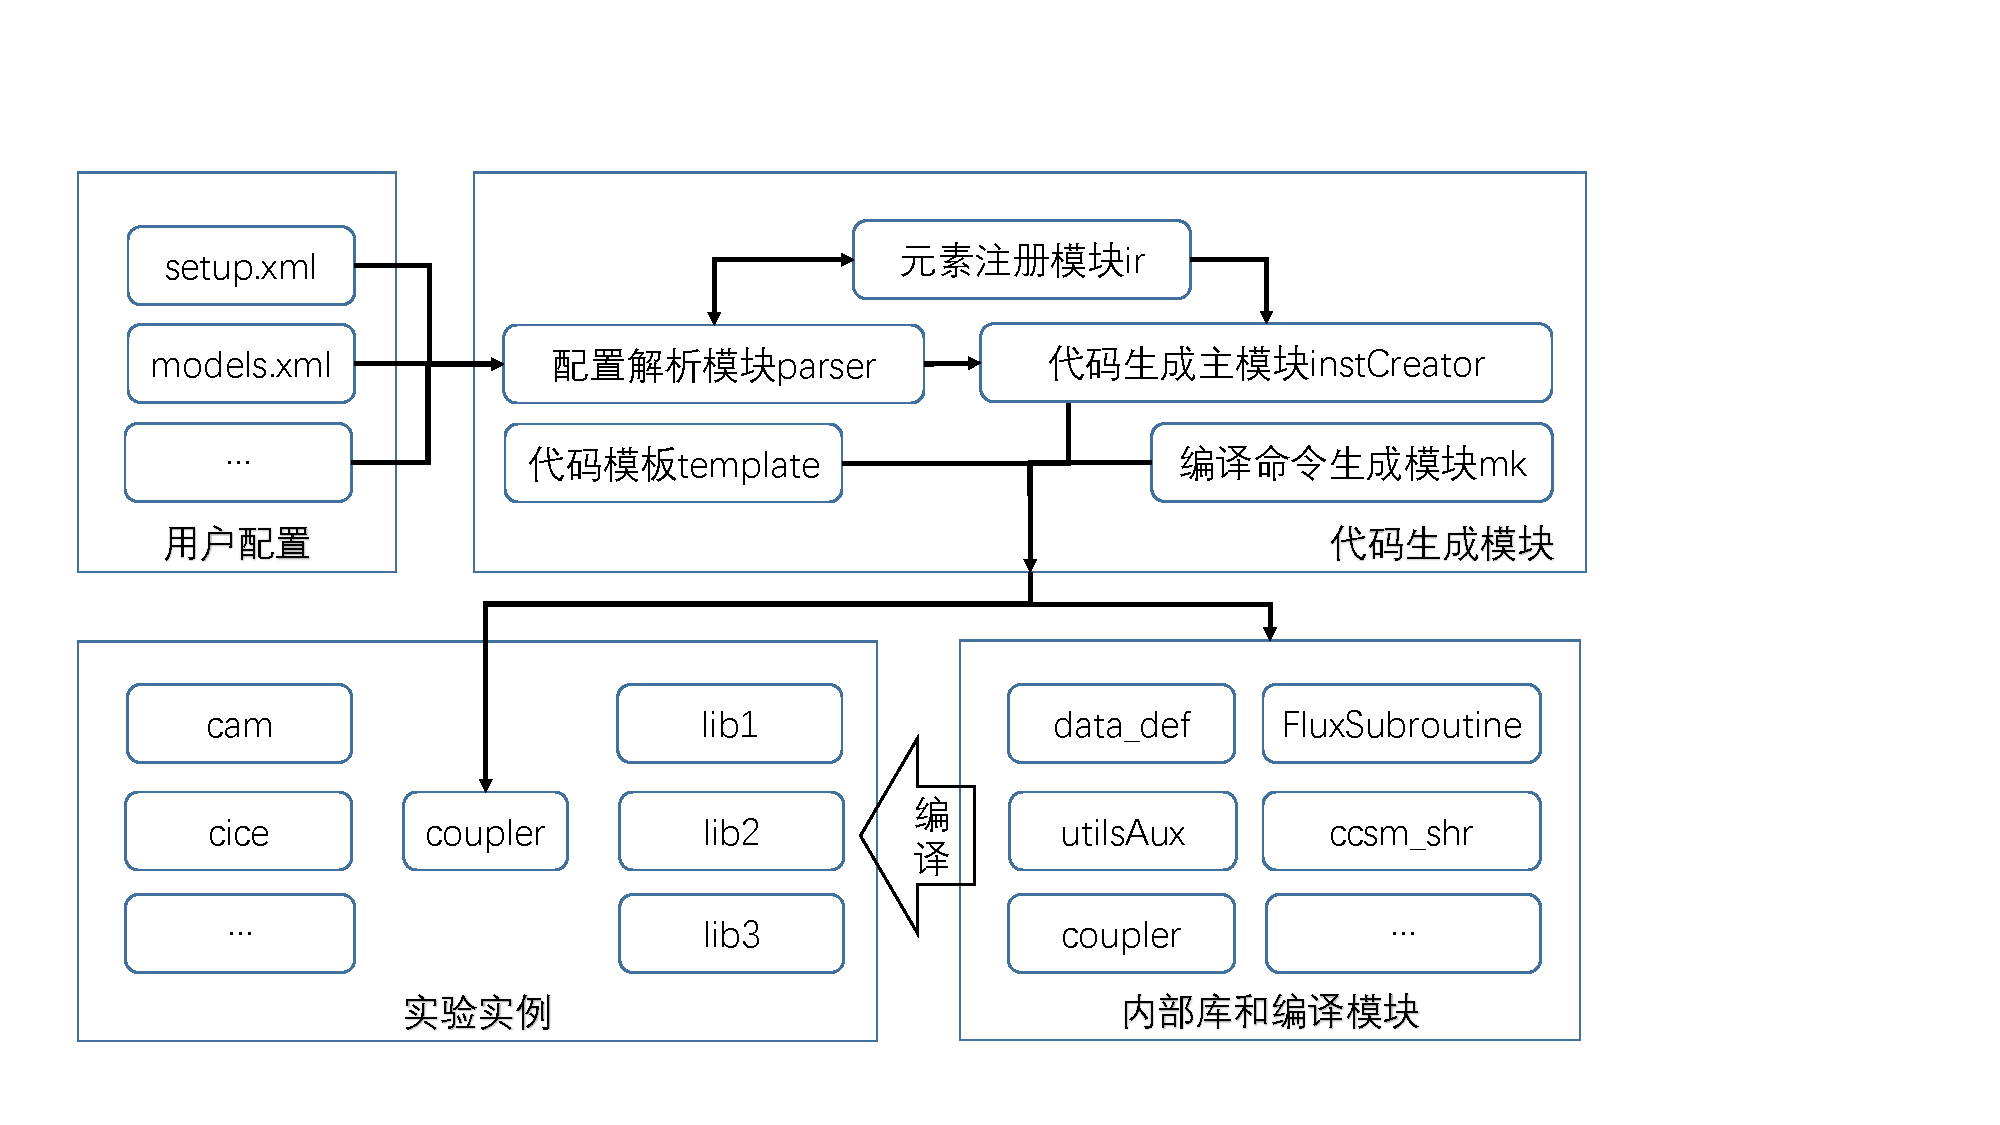
\includegraphics[width=1\textwidth]{../figures/fig1.pdf}
\caption{耦合平台运行流程图示例}
\end{figure}

\section{配置文件模块}

这部分是由用户提供的 xml 文件组成的配置集合。本文在适配各个模式分量实现的过程中对该部分的配置文件进行了规范化以降低用户配置的工作量和减少可能出现的错误配置和冗余导致的配置文件不一致。

在主要配置文件中,通过添加数据结构类型字段和网格比率类型字段,将不同类型的代码作为代码生成模块的内置函数自动生成,可以减少不同类型字段调用内部库函数时可能产生的冲突或错误。多个配置文件公用的分辨率、网格、接口类型等信息通过单独使用配置文件进行定义并通过短字符串代码进行引用的方式减少冗余和潜在的冲突或不一致可能。在配置文件中将各个模式分量独有的部分进行尽可能的隔离,并在共同接口处进行文件级引用,最大化各个模式分量实现的独立性,使得在将来多模式分量实现并行开发成为可能。简化了顶层耦合模块自身的配置文件,将部分相对固定的设置转移到编译选项和代码生成模块内部以精简配置文件和提高配置文件可读性。在外部文件引用模块中插入了默认的同网格映射配置,并在配置文件格式中区分了对内部不同数据结构可能存在的不同网格文件引用(虽然在目前用到的所有配置中这些文件都是相同的)以预备未来可能存在的高级设置。虽然本文目前的实验平台确定,本文还是提供了可配置的实验平台参数,该部分代码虽然未经过可扩展性测试,但在设计层面提供了原生跨平台的可能性。简化了伪模型的设计,省略了其与真模型相同但实质上无需配置的部分,使得对特定数据结构构造伪模型进行适配的时间成本一定程度上降低。将与物理过程相关的参数与代码实现相关的参数进行隔离,使得配置文件编写者可以专注于物理过程配置或代码层面配置。具体配置文件将会在下一章的实验结果中进行描述。

\section{代码生成模块}

这部分模块大部分为自动代码生成,对新加入的模式分量实现有较好的自动适配能力。这里主要是追加部分新功能和针对错误跟踪和调试进行结构上的修改。

\subsection{配置解析模块 parser}

该模块读入用户提供的 xml 配置文件并进行语法和语义检查,其中语法检查通过外部库来完成,而语义检查则通过内部自定义的 python 代码库完成。本文在调试模式开启时,将外部库的各个调用间插入了能够反映运行步骤的若干信息,从而可以在外部库发生错误的时候用代码生成模块内置的工具进行错误定位。在处理语义错误的情况时,本文通过与下面的元素注册模块配合以提前检查出部分冲突错误,并将可能的错误放在 ErrorHandler 模块下,通过多模块的协作将可能出现的错误在代码生成模块运行前即判明并尝试修复。另外,还修复了部分边界情况和空情况的处理,同时在这些情况下自动发出警告以避免配置文件编写错误。

\subsection{元素注册模块 ir}

由于部分模式分量自带一致性检测发现传输数据数量有误,追溯到配置解析模块发现耦合实验实例配置文件存在重复录入和局部名称冲突等问题。为了防止类似问题再次发生,在元素注册 ir 模块中加入了对各个数据域和跨模式分量的全局名称字典,在解析阶段即可进行全局冲突检测。这一步发生在代码生成之前,可以极大的节约编译运行和调试追溯时间。另外,针对部分很可能出现冲突的数据域,追加了可选用的顶层耦合内置前后缀的方式进行区分,降低了跨模式分量实现冲突可能。这一步操作需要内部库函数进行转译操作,且可能会导致在版本更新过程中带来的数据不一致问题,在最终进行数据分析时也要对外部工具进行修改,因此默认为关闭状态。

\subsection{代码生成主模块 instCreator}

这一部分本质上是通过 python 代码读取 xml 配置文件代码来生成 fortran 代码,这里需要大量的语义转换,最常见的就是 python 中的 True/False 和 fortran 中的 .true./.false. ,为了方便进行这些转换,本文在代码中添加了常见的翻译表,使得相同语义的不同语言表示可以在生成过程中自动切换。这在一定程度上减少编码复杂度,提高了代码可读性。需要注意的是这种语义自动转译需要配合转译字符使用,有较低概率会在用户编写特定文本时出现意料之外的转译,因此配合了日志模块和变异模块进行确认。

\subsection{编译命令生成模块 mk}

这部分可以通过耦合模式分量信息自动生成最终编译耦合实验主程序 coupler 的编译命令。通过各个模式分量自身的编译系统,所需的头文件和打包后的静态库文件被放置到设定的路径下,从而可以用相对路径找到。但对静态库的引用代码需要在编译命令生成模块中进行设置。为此,本文在输入的配置文件中加入了各个模式分量的输出命名规则,从而可以自动生成静态库链接代码,真正达成全自动生成和编译。

\section{内部库和编译模块}

这一部分的代码结构进行了调整,现在所有的 Makefile 进行了统一配置,其配置文件位于 baseCpl/src 目录下的 Makefile.conf 文件中,设置了 C++ 和 fortran 编译器及其主要依赖库的编译选项,包括 ESMF , NetCDF , ParallelIO 等外部库的头文件路径和库文件路径。与该模块相关的所有路径名称都要求设置为基于 ABSDIR 主目录宏的相对路径,这是为了在实验实例生成后路径变更时只需要对该宏进行自动修改即可在对应实例的目录下进行自动编译。各个依赖库的目录采用相对路径的方式对该配置文件进行引用,以确保在绝对路径改变后依然能够不依赖于宏地正确引用。

\subsection{数据定义模块 data\_def}

为了确保全局数据存储 global\_var 可以被多种模式分量实现用各自不同的方式进行访问和修改以提高适配面,降低适配难度,将所有分辨率修正前和修正后的数据结构对 MCT 的再封装进行展开,使得各个模式分量可以直接调用而不必通过顶层耦合模式进行解包,达成代码解耦的目的,同时也避免了多进程之间调用和多个模式分量实现之间可能存在的 race-condition 问题。

部分开关标记变量的副本转换为引用,牺牲少许效率换取原生的一致性。这一部分主要考虑到虽然顶层耦合模式存在多进程隔离的一致性保护,但各个模式分量实现编写过程中可能出现对这些变量的直接读取访问,这部分代码可能不受顶层耦合模式的隔离保护,因而可能会触发不一致的问题。值得一提的是,根据目前的框架和各个耦合模式分量的实现,并不存在将一个模式分量实现可写的数据暴露给另一个模式分量实现的情况,因此该设计仅为未来可能出现的该情况进行预先处理,在当前版本并未得到测试。

对通用宏进行了整合,现在默认字符串长度统一为 SHR\_KIND\_CS 和 SHR\_KIND\_CL 两个宏,这两个值在全局类型表文件 shr\_kind\_mod.F90 中被定义为所有不包含路径文本字符串的最大长度和全部文本字符串的最大长度,默认设为 80 和 256 个字符。在本修改前部分不带路径的文件名在 CESM 中被设定为 16 字符长度,因而出现了字符串溢出和命名冲突等问题。为此本文还插入了一个可选的字符串溢出检测模块,该模块开启时会对运行速度产生一定影响,但考虑到与字符串相关操作本身效率不高且已经被主要多进程运算部分尽可能避免,这部分实际测试中对运行效率的影响可以忽略不计,但仍然推荐在调试通过后的最终运行阶段关闭该模块。另外,本文对 CESM 中补充定义的 SHR\_KIND\_CX 和 SHR\_KIND\_CXX 两个宏进行了保留以方便其他模式分量的适配。这两个值预设为 512 和 4096。

\subsection{流数据传输模块 FluxSubroutine}

该模块用于不同模式分量实现中的数据传输时追加的适配数据处理。这部分代码涉及一定的物理运算,因此需要对调试工具进行适配从而可以检测出一个正确的模式分量输出在该模块由于数值溢出或误差等原因不满足目标模式分量输入的情况。另外,部分计算需要涉及到来自多个模式分量的多个数据结构,因此数据同步也要纳入错误检测范围内。实际上,在适配过程中出现了由于数据依赖关系复杂导致的运算顺序触发的错误,该错误在调试过程中无法被稳定复现,因此本文对该模块的调试模式加入了较强的同步要求以确保运行顺序不影响错误复现。

\subsection{输入合并模块 MrgSubroutine}

在加入新的模式分量实现后,需要根据其所需要的全部来自其他模式分量实现的数据编写输入合并模块,将这些数据整合进 run 模块的输入参数并进行必要的适配。考虑到各个模式分量对输入的处理存在较大差异,这部分代码没有采用代码生成模块自动进行生成而是要求用户自行编写。实际上,不共同模式分量实现的输入合并模块相似度很低,因此该设计并不增加各个模式分量适配的工作量,相反能够减少由于自动适配产生的接口冗余和可读性降低。与之相对的,该部分库函数代码所需的变量由代码生成模块处理并生成,使得人工编写该库函数时减少依赖变动。

\subsection{历史记录和存储恢复模块 utilsAux}

该模块调用 utils 进行文件读写,包括历史记录和存储恢复两部分。由于各个模块自身已有涉及这两个模块,且读写格式不统一,这里只处理顶层耦合模式可见的数据传输部分。来自各个模式分量的数据同名的情况通过插入来源模式分量名称进行区分,同时需要对后处理函数和数据分析工具进行调整。需要注意的是,经过顶层耦合模式的数据存在多种进程分配方式:按模式分量进程分配和按顶层耦合进程分配。他们所对应的全局分配表 GSMap 存在差异,需要用不同方式进行存储记录。这部分代码的更改主要是为了适配各种不同模式分量实现在数据存储上的不同情况而设置的多种输出过程。另外,为了使得顶层耦合模块可以正确输出模式分量实现自行配置的内容,需要在模式分量的 init 接口中对顶层耦合模块对应的数据接口配置文件进行设置,并由历史纪录和存储恢复模块进行读取以进行正确的对接和数据输出。

\subsection{CCSM 内置库模块 ccsm\_shr}

该模块存放了各个来源于 CCSM 的通用库函数,以备各个模式分量实现和顶层耦合模式中保留的来源于 CESM 的代码进行调用。由于该部分被完整地应用于 CESM 实际运行的实例中,因此正确性可以得到保证,但在本文适配的过程中可能会出现各种数据不匹配的情况,从而在调用正确的库函数过程中发生错误,从而定位到 ccsm\_shr 模块内部。因此,本文并不将这部分代码视作黑盒,而是在适当位置插入调试信息和数据追溯,以确保在该模块内部发生的异常可以较为容易的追溯到数据结构来源,从而达到提高调试效率的目的。同时,考虑到未来顶层耦合模式的更新对该模块进行可能的更改和再封装,又要和原版模式分量保持兼容性,本文对于重封装函数保留了原版接口。


\chapter{实验结果}
\label{cha:experiment}

在本章中,我们完整地展示了 F2000 模式分量的代码生成、编译、运行、数据分析等步骤。

\section{配置文件}

\usetikzlibrary{trees}
\tikzstyle{every node}=[draw=black,thick,anchor=west]
\tikzstyle{selected}=[draw=red,fill=red!30]
\tikzstyle{optional}=[dashed,fill=gray!50]

\begin{figure}[H]
\begin{tikzpicture}[%
  grow via three points={one child at (0.5,-0.7) and
  two children at (0.5,-0.7) and (0.5,-1.4)},
  edge from parent path={(\tikzparentnode.south) |- (\tikzchildnode.west)}]
  \node{models}
  child { node {model}
    child { node {name}
      child {node {atm}}
    }
    child [missing] {}
    child { node {version}
      child {node {cam}}
    }
    child [missing] {}
    child { node {attrVect}
      child {node {...}}
    }
    child [missing] {}    
    child { node {domain}
      child {node {...}}
    }
    child [missing] {}    
    child { node {method}
      child {node {init}
        child { node {name}
        	child { node {atm\_init\_mct}}
        }
        child [missing] {}
        child { node {in\_args}
          child { node {arg}
            child { node {atm2x\_atmatm}}
          }
        }
        child [missing] {}
        child [missing] {}
        child { node {out\_args}
          child { node {arg}
            child { node {x2atm\_atmatm}}
          }
        }
        child [missing] {}
        child [missing] {}
      }
      child [missing] {}
      child [missing] {}
      child [missing] {}
      child [missing] {}
      child [missing] {}
      child [missing] {}
      child {node {run}
        child { node {...} }
      }
      child [missing] {}    
      child {node {final}
        child { node {...} }
      }
      child [missing] {}    
    }
  }
  child [missing] {}    
  child [missing] {}    
  child [missing] {}    
  child [missing] {}    
  child [missing] {}    
  child [missing] {}    
  child [missing] {}    
  child [missing] {}    
  child [missing] {}    
  child [missing] {}    
  child [missing] {}    
  child [missing] {}    
  child [missing] {}    
  child [missing] {}    
  child [missing] {}    
  child [missing] {}    
  child [missing] {}    
  child [missing] {}    
  child { node {model}
    child { node {name}
      child { node {ocn} }
    }
    child [missing] {}
    child { node {...} }
  }
  child [missing] {}
  child [missing] {}
  child [missing] {}
  child {node {...}};
\end{tikzpicture}
\caption{models.xml 结构示意图}
\end{figure}


\begin{figure}[H]
\begin{tikzpicture}[%
  grow via three points={one child at (0.5,-0.7) and
  two children at (0.5,-0.7) and (0.5,-1.4)},
  edge from parent path={(\tikzparentnode.south) |- (\tikzchildnode.west)}]
  \node {setup}
    child { node {models} 
      child { node {model}
        child { node {name}
          child { node {atm} }
        }
        child [missing] {}
        child { node {version}
          child { node {cam} }
        }
        child [missing] {}    		
        child { node {res}
          child { node {fv4x5} }
        }
        child [missing] {}
        child { node {frac [update=true]}
          child { node {normal} }
        }
        child [missing] {}
        child { node {input}
          child { node {src [name='ocn']} 
          	child { node {field [type='state' frac='normal']}
          	  child {node {So\_t}}
          	}
          	child [missing] {}          	
          }
          child [missing] {}
          child [missing] {}
          child { node {src [name='lnd']} 
          	child { node {field [type='state' frac='normal']}
          	  child {node {Sl\_fv:Sl\_ram1:...}}
          	}
          	child [missing] {}          	
          }
          child [missing] {}
          child [missing] {}
          child { node {src [name='ice']} 
          	child { node {field [type='state' frac='normal']}
          	  child {node {Si\_avsdr}}
          	}
          	child [missing] {}          	
          }
          child [missing] {}
          child [missing] {}          
          child { node {src [name='xao' type='var']} 
          	child { node {var}
          	  child {node {xao\_ax}}
          	}
          	child [missing] {}      	
          }
          child [missing] {}
          child [missing] {}        }
        child [missing] {}
      }
      child [missing] {}
      child [missing] {}
      child [missing] {}
      child [missing] {}
      child [missing] {}
      child [missing] {}
      child [missing] {}
      child [missing] {}
      child [missing] {}
      child [missing] {}
      child [missing] {}
      child [missing] {}
      child [missing] {}
      child [missing] {}
      child [missing] {}
      child [missing] {}
      child [missing] {}
      child [missing] {}
      child [missing] {}
      child [missing] {}
      child [missing] {}
      child [missing] {}
      child [missing] {}
      child { node {model}
        child { node {name}
          child { node {ocn} }
        }
        child [missing] {}
        child { node {...} }
      }
      child [missing] {}
      child [missing] {}
      child [missing] {}
      child { node {...} } 
    };
\end{tikzpicture}
\caption{setup.xml 结构示意图}
\end{figure}

\begin{figure}[H]
\begin{tikzpicture}[%
  grow via three points={one child at (0.5,-0.7) and
  two children at (0.5,-0.7) and (0.5,-1.4)},
  edge from parent path={(\tikzparentnode.south) |- (\tikzchildnode.west)}]
  \node{option}
  child{ node {time}
    child { node {calendar type='string'}
      child { node {NO\_LEAP} }
    }
    child [missing] {}
    child { node {stop\_option type='string'}
      child {node {ndays}}
    }
    child [missing] {}
    child { node {stop\_n type='int'}
      child {node {10}}
    }
    child [missing] {}
    child { node {stop\_ymd type='int'}
      child {node {20010301}}
    }
    child [missing] {}
    child { node {restart\_option type='string'}
      child {node {ndays}}
    }
    child [missing] {}
    child { node {restart\_n type='int'}
      child {node {5}}
    }
    child [missing] {}
    child { node {restart\_ymd type='int'}
      child {node {-1}}
    }
    child [missing] {}
    child { node {history\_option type='string'}
      child {node {ndays}}
    }
    child [missing] {}
    child { node {...}}
    child { node {start\_ymd type='int'}
      child {node {20010101}}
    }
    child [missing] {}
    child { node {start\_tod type='int'}
      child {node {0}}
    }
    child [missing] {}
    child { node {ref\_ymd} }
    child { node {comps}
      child {node {atm\_cpl\_dt}
        child {node {3600}}
      }
      child [missing] {}
      child {node {ocn\_cpl\_dt}
        child {node {86400}}
      }
      child [missing] {}
      child {node {...} }
    }
    child [missing] {}
    child [missing] {}
    child [missing] {}
    child [missing] {}
    child [missing] {}
    child { node {end\_restart type='bool'}
      child {node {.false.}}
    }
  };
\end{tikzpicture}
\caption{option.xml 结构示意图}
\end{figure}

\begin{figure}[H]
\begin{tikzpicture}[%
  grow via three points={one child at (0.5,-0.7) and
  two children at (0.5,-0.7) and (0.5,-1.4)},
  edge from parent path={(\tikzparentnode.south) |- (\tikzchildnode.west)}]

  \node{field}
  child { node {fieldMeta}
  child { node {fields}
    child { node {fieldVar name='flds\_doom\_coord'}
    	child { node {lat:lon} }
    }
    child [missing] {}
    child { node {fieldVar name='flds\_doom\_other'}
    	child { node {area:aream:mask:frac} }
    }
    child [missing] {}
    child { node {...} }
  }
  child [missing] {}
  child [missing] {}
  child [missing] {}
  child [missing] {}
  child [missing] {}
  child { node {fldMeta}
    child { node {fld}
      child { node {shortname}
        child {node {lat}}
      }
      child [missing] {}
      child { node {longname}
        child {node {unknown}}
      }
      child [missing] {}
      child { node {stdname}
        child {node {latitude}}
      }
      child [missing] {}
      child { node {units}
        child {node {degrees north}}
      }
      child [missing] {}
    }
    child [missing] {}
    child [missing] {}
    child [missing] {}
    child [missing] {}
    child [missing] {}
    child [missing] {}
    child [missing] {}
    child [missing] {}
    child { node {fld}
      child { node {shortname}
        child {node {Sa\_u}}
      }
      child [missing] {}
      child { node {longname}
        child {node {Zonal wind at the lowest model level}}
      }
      child [missing] {}
      child { node {stdname}
        child {node {eastward\_wind}}
      }
      child [missing] {}
      child { node {units}
        child {node {m s-1}}
      }
      child [missing] {}
    }
    child [missing] {}
    child [missing] {}
    child [missing] {}
    child [missing] {}
    child [missing] {}
    child [missing] {}
    child [missing] {}
    child [missing] {}
    child { node {...}}
  }
  };
\end{tikzpicture}
\caption{fields.xml 结构示意图}
\end{figure}

\begin{figure}[H]
\begin{tikzpicture}[%
  grow via three points={one child at (0.5,-0.7) and
  two children at (0.5,-0.7) and (0.5,-1.4)},
  edge from parent path={(\tikzparentnode.south) |- (\tikzchildnode.west)}]

  \node{fakeModel}
    child { node {models}
    	child { node {model type='fake'}
    		child { node {name}
    			child {node {xao}}
    		}
    		child [missing] {}
    		child { node {fields}
    			child {node {flds\_xao\_states,flds\_xao\_fluxes,...}}
    		}
    		child [missing] {}
    		child { node {deps}
    			child {node {atm:ocn}}
    		}
    		child [missing] {}
    		child { node {variables}
    			child {node {variable type='attrVect'}
    				child { node {name}
    					child {node {xao\_ox}}
    				}
		    		child [missing] {}
    				child { node {grid}
    					child {node {ocn}}
    				}
		    		child [missing] {}
		    		child { node {method}
		    			child { node {init}
		    				child {node {...}}
		    			}
		    			child [missing] {}
		    			child { node {run}
		    				child {node {...}}
		    			}
		    			child [missing] {}
		    			child { node {final}
		    				child {node {...}}
		    			}
		    			child [missing] {}
		    		}
		    		child [missing] {}
		    		child [missing] {}
		    		child [missing] {}
		    		child [missing] {}
		    		child [missing] {}
		    		child [missing] {}
    			}
	    		child [missing] {}
	    		child [missing] {}
	    		child [missing] {}
	    		child [missing] {}
	    		child [missing] {}
	    		child [missing] {}
	    		child [missing] {}
	    		child [missing] {}
	    		child [missing] {}
	    		child [missing] {}
	    		child [missing] {}
    			child {node {variable type='attrVect'}
    				child { node {name}
    					child {node {xao\_ax}}
    				}
		    		child [missing] {}
    				child { node {grid}
    					child {node {atm}}
    				}
		    		child [missing] {}
		    		child { node {...} }
    			}
	    		child [missing] {}
	    		child [missing] {}
	    		child [missing] {}
	    		child [missing] {}
	    		child [missing] {}
    			child {node {...}}
    		}
    	}
   		child [missing] {}
   		child [missing] {}
   		child [missing] {}
   		child [missing] {}
   		child [missing] {}
   		child [missing] {}
   		child [missing] {}
   		child [missing] {}
   		child [missing] {}
   		child [missing] {}
   		child [missing] {}
   		child [missing] {}
   		child [missing] {}
   		child [missing] {}
   		child [missing] {}
   		child [missing] {}
   		child [missing] {}
   		child [missing] {}
   		child [missing] {}
   		child [missing] {}
   		child [missing] {}
   		child [missing] {}
   		child [missing] {}
   		child [missing] {}
   		child [missing] {}
   		child [missing] {}
   		child { node {...} }
    };
\end{tikzpicture}
\caption{fakeModel.xml 结构示意图}
\end{figure}

以上是用户输入的配置文件的主要部分,分别对应 models.xml , setup.xml , option.xml , field.xml ,  fakeModel.xml 五个配置文件。由于篇幅所限部分域用省略号 ... 代替,其余配置文件请参见 github 代码库 \footnote{https://github.com/NeoGeon/BCGen} 。

\section {代码生成}

在用户配置全部录入后,可以通过代码生成模块中的 instCreator 模块进行解析和代码生成。该模块会将解析出的结果以 log 的形式输出到屏幕。若配置正确,应当会产生如下输出:

\begin{lstlisting}
('name', 'atm2x_atmx')
('model', 'atm')
('fraclist', 'afrac:ofrac:lfrac:ifrac')
('init', 'fraction_atm_init')
('update', 'fraction_atm_update')
{'fraclist': 'afrac:ofrac:lfrac:ifrac', 
'init': 'fraction_atm_init', 'update': 
'fraction_atm_update', 'fracs': [{'mapper': 
'mapper_Smatocn2atm', 'model': 'ocn', 'name': 
'ofrac'}, {'mapper': 'mapper_Smatlnd2atm',
'model': 'lnd', 'name': 'lfrac'}, {'mapper':
'mapper_Smatice2atm', 'model': 'ice',
'name': 'ifrac'}]}
...
('name', 'mapper_comp_map')
('arg', 'ocn2x_ocnx')
('arg', 'ocn2x_atmx')
('attrVect', 'lnd2x_lndx')
('field', 'Sl_fv:Sl_ram1:Sl_snowh:Fall_flxdst1:
Fall_flxdst2:Fall_flxdst3:Fall_flxdst4')
...
\end{lstlisting}

\section {内部库预编译}

全部代码生成后会调用 make 工具进行自动内部库编译,若内部库和生成代码格式正确且接口符合,应当会产生如下输出

\begin{lstlisting}
make[1]: Entering directory `/home/hq/git
/protected/BCGen/baseCpl/src/logUtils'
mpif90 -c -I/home/hq/git/protected/BCGen/
baseCpl/include -L/home/hq/git/protected/
BCGen/baseCpl/lib logUtil.F90 
mv *.o /home/hq/git/protected/BCGen/baseCpl/lib
mv *.mod /home/hq/git/protected/BCGen/baseCpl/include
make[1]: Leaving directory 
...
Checking whether input datasets exist locally...
OK -- found depvel_file = /mnt/CESM-data/inputdata/
atm/cam/chem/trop_mozart/dvel/depvel_monthly.nc
OK -- found tracer_cnst_filelist = /mnt/CESM-data/
inputdata/atm/cam/chem/trop_mozart_aero/oxid/
oxid_1.9x2.5_L26_clim_list.c090805.txt
...
\end{lstlisting}

\section {生成实例}

编译后的内部库会与各个模式分量实现的代码一同创建为实验实例,其结构如下图。该实例可以直接编译运行,或对模式分量实现进行嵌入式调试。

\begin{figure}[H]
\begin{tikzpicture}[%
  grow via three points={one child at (0.5,-0.7) and
  two children at (0.5,-0.7) and (0.5,-1.4)},
  edge from parent path={(\tikzparentnode.south) |- (\tikzchildnode.west)}]

  \node{BCGen}
    child { node{BCGen\_inst}
    	child { node {include} 
    		child { node {这里存放内部库和各个模式分量实现的.mod文件} }
    	}
    	child [missing] {}
    	child { node {lib}
    		child { node {这里存放内部库和各个模式分量实现的.o和.a文件} }
    	}
    	child [missing] {}
    	child { node {scripts}
    		child { node {instBuild.sh 自动编译脚本} }
    		child { node {pullDeps.py 自动更新依赖脚本} }
    	}
    	child [missing] {}
    	child [missing] {}
    	child { node {src}
    		child { node {mapper.rc 部分数值文件列表}}
    	}
    	child [missing] {}
    	child { node {models}
    		child { node {cpl}
    			child { node {耦合器主代码,可自动编译为可执行文件} }
    		}
    		child [missing] {}
    		child { node {atm}
    			child { node {大气模式分量实现} }
    		}
    		child [missing] {}
    		child { node {ocn}
    			child { node {海洋模式分量实现} }
    		}
    		child [missing] {}
    		child { node {...} }
    	}
    };
\end{tikzpicture}
\caption{生成实例结构示意图}
\end{figure}

\section {数据分析}

通过 ncl\footnote{http://www.ncl.ucar.edu/Applications/maponly.shtml} 语言对输出的 NetCDF 数据进行作图,可以得出可视化结果。以下为其中一例数据结构:

\begin{figure}[H]
\centering
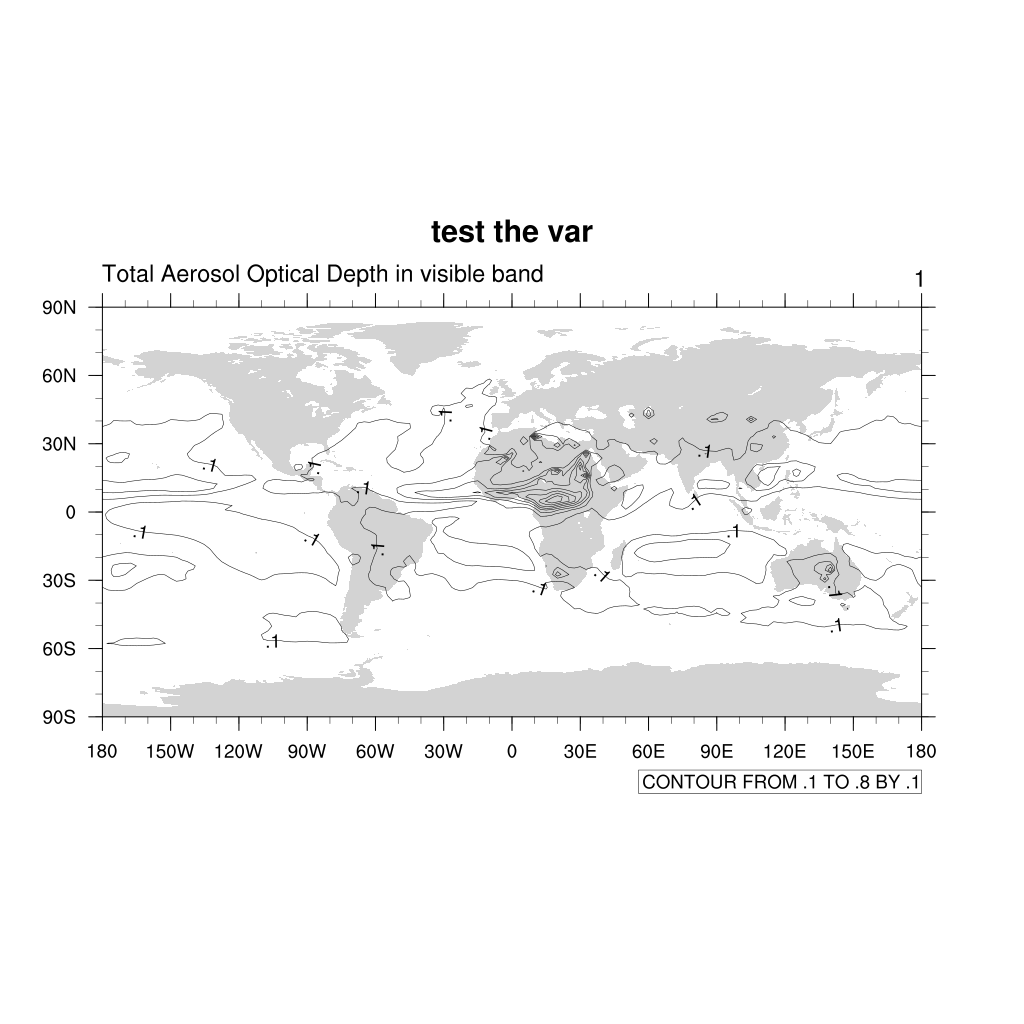
\includegraphics[width=1\textwidth]{../figures/test.png}
\caption{数据分析结果图}
\end{figure}



%%% 其它部分
\backmatter

%% 本科生要这几个索引,研究生不要。选择性留下。
% 插图索引
\listoffigures
% 表格索引
\listoftables
% 公式索引
\listofequations


%% 参考文献
% 注意:至少需要引用一篇参考文献,否则下面两行可能引起编译错误。
% 如果不需要参考文献,请将下面两行删除或注释掉。
\bibliographystyle{thuthesis-numeric}      % 顺序编码制
% \bibliographystyle{thuthesis-author-year}  % 著者-出版年制
% \bibliographystyle{thuthesis-bachelor}     % 本科生参考文献的著录格式
\bibliography{ref/refs}


%% 致谢
% 如果使用声明扫描页,将可选参数指定为扫描后的 PDF 文件名,例如:
% \begin{acknowledgement}[scan-statement.pdf]
\begin{acknowledgement}
  衷心感谢导师 黄震春 副研究员和计算机系 钟安润 学长对本人的精心指导。他们的言传身教将使
  我终生受益。

  感谢 \LaTeX 和 \thuthesis\cite{thuthesis},帮我节省了不少时间。
\end{acknowledgement}


%% 附录
\begin{appendix}
\chapter{开题报告暨相关外文资料调研阅读报告}

\section{项目背景}

CESM模型是一类应用较为广泛的自然气候变化模型,它包括大气模型,陆地模型,海洋模型等子模型。每个模型主要内容为求解偏微分方程,而不同子模型间互相提供边界值。近年来由于各种新模型的不断衍生,存在将不同子模型进行对比的需求。而原本CESM的代码内部依赖逻辑较为复杂,使得将子模型切分并重组较为困难。为了解决这个问题,耦合器定义了一套标准接口,并将各个子模型切分开来运用这一套接口独立运行,再通过耦合器内部进行边界值通信,最终得以复现原本CESM模型的运行,从而使得更换子模型进行对比变得较为简单。目前学长即将完成耦合器的第一版编写,我的当前任务是将第一个大气模型CAM配置运行成功,并将其拆解依赖后重新封装为耦合器标准接口库。为此,我阅读了CESM论文\cite{OPENCESM} ,CAM论文 \cite{OPENCAM} ,以及与我之后的研究方向:耦合器通信相关的MCT论文 \cite{OPENMCT1} \cite{OPENMCT2}。

\section{CESM论文阅读报告}

论文:

THE COMMUNITY EARTH SYSTEM MODEL (CESM) LARGE ENSEMBLE PROJECT A Community Resource for Studying Climate Change in the Presence of Internal Climate Variability by J. E. Kay, C. Deser, A. Phillips, A. Mai, C. Hannay, G. Strand, J. M. Arblaster, S. C. Bates, G. Danabasoglu, J. Edwards, M. Holland, P. Kushner, J.-F. Lamarque, D. Lawrence, K. Lindsay, A. Middleton, E. Munoz, R. Neale, K. Oleson, L. Polvani, and M. Vertenstein

概要:

CESM是一个研究非受迫气候变化的模型,其主要目的是通过内部气候变化研究对气候预测提供参考。CESM包含大气子模型,海洋子模型,陆地子模型,极地子模型等,并可以求解其耦合作用。其设计动机是各个子模型通常只能考虑到单个方面因素的作用,因而受到其他方面因素的影响较大且难以控制模型误差,因此考虑把多个模型联合求解。文章主要作为CESM模型的文档和简要实验结果。

不同模型有着不同的迭代周期,这是因为洋流在长达几千年的时间跨度上的变化几乎不会影响模型结果,但大气,陆地和极地收到外部环境影响较为严重,需要短至每数周长至一年就要更新外部观测数据。

模型共进行了30个实验,除去2个实验作为对照组之外,剩下28个实验使用完全相同的外部数据和带有微小误差的初始值数据,来通过统计对模型的误差和置信度进行估计。从结果上看,这些模型对全球变暖程度的预估在合理范围内,从而证明了内部气候变化对气候预测能够起到一定的作用。

CESM模型的分辨率通常较低,这一方面是因为计算复杂度受限,另一方面则是由于模型精度导致。在局部地区实验中,只有微小误差的原始数据在不同模型中得到了截然不同的结果(气温相差接近1万度)。这一定程度上反映了气候变化中的蝴蝶效应,同时也说明了内部气候变化预测的局限性。为了解决这一问题,一些针对特定地区建立的高分辨率子模型逐渐被开发出来。它们通过毗邻的低分辨率模型作为初值进行迭代求解,并通过其自身的高分辨率尽可能缩小误差。预测时间被缩短以减少蝴蝶效应的影响,同时区域面积的缩小也使得提高分辨率的模型依然可以在可接受的时间内得出结果。

文章对比了CESM和CMIP5模型。CMIP5的不同模型采用了不同的公式,而CESM模型控制外部参数不变,只有初值有微量的误差,因而在控制变量方面做的更好,可以得出更加有说服力的结论。


气候预测的一个重要目的是预测极端天气。而由于分辨率低下的原因,通常的模型对极端天气的适应度并不好。因此,CESM将极端天气作为外部因素输入到模型中,使得模型可以更加关注和拟合通常情况的气候变化。

总的来说,CESM对建立新的子模型提供了大量的外部参数处理和误差分析工作,使得一个具有局限的模型可以接入CESM而得出较为可靠的结果。

CESM的设计初衷和本文现在试图进行的实验相似度很高。然而本质的不同是,CESM注重于解决模型在理论计算上的局限性,编写者大多为研究气候、地理的科学家,而本文将要实现的耦合器注重于降低接入新模型的工作量,即将这些科学家写的代码转化为成体系的库。

\section{CAM论文阅读报告}

论文:

Exploratory High-Resolution Climate Simulations using the Community Atmosphere Model (CAM) JULIO T. BACMEISTER Atmospheric Modeling and Prediction Section, National Center for Atmospheric Research,* Boulder, Colorado MICHAEL F. WEHNER Lawrence Berkeley National Laboratory, Berkeley, California RICHARD B. NEALE, ANDREW GETTELMAN, CECILE HANNAY, PETER H. LAURITZEN, JULIE M. CARON, AND JOHN E. TRUESDALE Atmospheric Modeling and Prediction Section, National Center for Atmospheric Research,* Boulder, Colorado


概要:

CAM是CESM模型中被广泛采用的大气子模型。文章主要对比不同分辨率下模型的结果精度,以及提出了一种针对热带气旋的分布模型和复现热带气旋的一些技巧。文章讲述了CAM模型的参数调节,实验步骤,输入数据,以及针对高分辨率的一些调整。文章还叙述了一些特定的气候现象以及捕捉它们所需的分辨率,并针对这些气候现象建立了基础模型。最后,文章对一些特定时间和特定区域的实验进行了说明。

由于具体公式只影响模型本身,而对于耦合器来说模型计算部分可以看作黑箱,本文只需要关心模型的外部输入,参数设定和边界值传递,因此公式部分暂且略过。

从实验结果来看,高分辨率模型的降水概率提高,这是因为高分辨率模型捕捉到了更多的降雨事件,但从总体来看平均降雨量并没有发生显著变化。这意味着统计降雨量并不需要过高分辨率的模型,但高分辨率模型可以更加精确的预测某个特定位置是否降雨。这说明了不同目标对不同模型的需求。

针对不同季节的模型测试中发现,不同季节可能会产生不同种类的天气现象,而并没有一个模型能同时很好地观测全部这些天气现象。因此,较为科学合理的方式是分别采用针对各个天气进行特化的模型对每个时间段进行迭代。

在针对美国的一些特殊极端天气情况的测试中,提高分辨率可以在冬季捕捉到更多的极端天气,但在夏天的表现和低分辨率模型并无显著差异。特别的,对于热带气旋,无论是否提高分辨率,模型都无法准确地区分两个气旋。这说明不同时间段可以采用不同的分辨率模型。

为了更好的识别气旋,文章分析了CAM5的数据,分析了它对气旋识别不理想的原因,并针对性地设计了新模型。虽然结果看起来依旧不足以令人满意,但一定程度上减小了误差。这要求整个模型应当能够较为方便地分析每个子模型的数据,为设计新模型提供参考。

总的来说,CAM作为CESM中比较有代表性的一个模块,它的实验流程中遇到的需求对本文设计耦合器有较大的指导意义。

\section{MCT论文阅读报告}

论文1:

M × N COMMUNICATION AND PARALLEL INTERPOLATION IN COMMUNITY CLIMATE SYSTEM MODEL VERSION 3 USING THE MODEL COUPLING TOOLKIT Robert Jacob Jay Larson Everest Ong

论文2:

THE MODEL COUPLING TOOLKIT: A NEW FORTRAN90 TOOLKIT FOR BUILDING MULTIPHYSICS PARALLEL COUPLED MODELS Jay Larson Robert Jacob Everest Ong

	由于MCT要求同时引用这两篇文章,因此我同时阅读了这两篇。其中第一篇主要从算法层面讲述了MCT,而第二篇主要从接口和代码抽象方面给出了文档。

	MCT设计初衷是服务于CESM的各子模型通信交换。CESM通信交换的最初实现是通过一个单线程耦合器分别与多个模型通信来交换外界参数,但随着CESM分辨率提高,所需的线程数也逐步增加,单线程耦合器将会成为瓶颈。因而多线程与多线程间的通信需求成为必要。

	MCT主要解决的是CESM各模块间的通信问题,其模型可以抽象为A模型的m个进程与B模型的n个进程进行通信,而通信数据在两个模型分辨率相同时为p*q的网格,分辨率不同时为p1*q1,p2*q2的网格且需要将传输的数据进行插值。

	接口方面,MCT直接用同类接口替代CESM中的MPI,以最大化地保持原本代码结构和可移植性。MCT定义了两种主要类型AttributeVector和GSMap,前者为一个二维数组用于存储实数数据,而后者用于记录这些数据分别属于哪些进程。虽然每个子模型实现方式各不相同,但它们的数据都可以通过这两种主要类型进行记录和传递,从而满足了可扩展性。

	在数据传递算法中,首先考虑不需要插值的情况,即两个模型的分辨率和网格完全相同。MCT采用一个Router模块记录了每个网格点在另一个模型中属于哪个线程,这个模块可以在两个模型交换GSMap之后各自并行建立,并在初始化后不再改变。Router建立后即可开始进程并行的传输。为了减小通信碎片,在每个发送线程的一对多传输中,所有消息一起发送,并在接收端拆分。

	接下来考虑需要插值的情况。插值可以通过一个矩阵乘法实现,而由于实际模型中网格内有大量0值点,MCT提供了稀疏矩阵存储和乘法来提高插值效率。对稀疏矩阵进行并行乘法时,MCT提供了按矩阵行(源)和矩阵列(目标)拆分并行两种计算方式。在传输时,前者需要在传输前进行插值计算再利用同网格的数据传输算法发送插值后的数据,而后者应当把数据传输到目标模型后再插值计算。由于网格数据格式和插值所需格式不同,MCT提供了Rearrange模块用于改变数据格式以提高插值效率。

	文章进行了各个模块参数的实验和比较,并得出了在当时CESM模型下的一组最优解。从耦合器的设计角度考虑,本文需要更换各种子模型进行实验,而对每个模型应当有不同的最优效率参数。因此,本文将配置格式化为xml文件并利用耦合器自动生成代码,这样可以针对每一组新模型较为方便地测试出一组较优的配置并运行求解。

\section{总结}

开题阶段,在导师和学长的指导和帮助下,我阅读了上述论文,初步了解了实验背景和基准算法,并对研究方向和优化目标有了初步的认识。

\end{appendix}

%% 个人简历
\begin{resume}

  \resumeitem{个人简历}

  1996 年 11 月 2 日出生于 天津 市 河北 区。

  2015 年 9 月免试进入 清华 大学 计算机科学与技术 系,攻读 学士 学位至今。

\end{resume}


%% 本科生进行格式审查是需要下面这个表格,答辩可能不需要。选择性留下。
% 综合论文训练记录表
\includepdf[pages=-]{scan-record.pdf}
\end{document}
